\documentclass[12pt]{article}
\usepackage{hyperref}
\usepackage{listings}
\usepackage[margin=1in]{geometry}
\usepackage{enumitem}
\usepackage{multicol}
\usepackage{array}
\usepackage{titlesec}
\usepackage{helvet}
\renewcommand{\familydefault}{\sfdefault}
\usepackage{amsmath}     % For math equations
\usepackage{amssymb}     % For advanced math symbols
\usepackage{amsfonts} % For math fonts
\usepackage{gvv}
\usepackage{esint}
\usepackage[utf8]{inputenc}
\usepackage{graphicx}
\usepackage{pgfplots}
\pgfplotsset{compat=1.18}
\titleformat{\section}{\bfseries\large}{\thesection.}{1em}{}
\setlength{\parindent}{0pt}
\setlength{\parskip}{6pt}
\usepackage{multirow}

\usepackage{fancyhdr}     % For custom headers and footers

\pagestyle{fancy}         % Use the fancy page style
\fancyhf{}                % Clear existing header/footer

% Header customization
\renewcommand{\headrulewidth}{0.4pt}          % Horizontal line at top
\fancyhead[L]{\textbf{GATE 2024}}                       % Page number on left
\fancyhead[R]{\textbf{ENGINEERING SCIENCES – XE}}  % Custom text on right
\cfoot{\thepage}

\usepackage[siunitx,RPvoltages]{circuitikz}
\usepackage{tikz}
\usepackage{float}
\usepackage{caption}

\begin{document}

\begin{center}
    {\Large \textbf{GA - GENERAL APTITUDE}}
\end{center}



\begin{enumerate}

\item[] \textbf{Q1 - Q5 carry one mark each.}
\item If `$\rightarrow$' denotes increasing order of intensity, then the meaning of the words [walk $\rightarrow$ jog $\rightarrow$ sprint] is analogous to [bothered $\rightarrow$ \_\_\_\_\_ $\rightarrow$ daunted].  

Which one of the given options is appropriate to fill the blank?
\begin{enumerate}
\item phased
\item phrased
\item fazed
\item fused
\end{enumerate}
(GATE XE 2024)

\item Two wizards try to create a spell using all the four elements, \textit{water, air, fire}, and \textit{earth}. For this, they decide to mix all these elements in all possible orders. They also decide to work independently. After trying all possible combination of elements, they conclude that the spell does not work.  

How many attempts does each wizard make before coming to this conclusion, independently?
\begin{enumerate}
\item 24
\item 48
\item 16
\item 12
\end{enumerate}
(GATE XE 2024)

\item In an engineering college of 10,000 students, 1,500 like neither their core branches nor other branches. The number of students who like their core branches is $\tfrac{1}{4}$ of the number of students who like other branches. The number of students who like both their core and other branches is 500.  

The number of students who like their core branches is
\begin{enumerate}
\item 1,800
\item 3,500
\item 1,600
\item 1,500
\end{enumerate}
(GATE XE 2024)

\item For positive non-zero real variables $x$ and $y$, if
$$
\ln\!\left(\frac{x+y}{2}\right) = \frac{1}{2}\,[\ln(x) + \ln(y)]
$$
then, the value of $\dfrac{x}{y} + \dfrac{y}{x}$ is
\begin{enumerate}
\item 1
\item $\tfrac{1}{2}$
\item 2
\item 4
\end{enumerate}
(GATE XE 2024)

\item In the sequence $6, 9, 14, x, 30, 41$, a possible value of $x$ is  
\begin{enumerate}
\item 25
\item 21
\item 18
\item 20
\end{enumerate}
(GATE XE 2024)

\item[] \textbf{Q6 - Q10 carry two marks each.}
\item Sequence the following sentences in a coherent passage.  

P: This fortuitous geological event generated a colossal amount of energy and heat that resulted in the rocks rising to an average height of 4 km across the contact zone.  

Q: Thus, the geophysicists tend to think of the Himalayas as an active geological event rather than as a static geological feature.  

R: The natural process of the cooling of this massive edifice absorbed large quantities of atmospheric carbon dioxide, altering the earth's atmosphere and making it better suited for life.  

S: Many millennia ago, a breakaway chunk of bedrock from the Antarctic Plate collided with the massive Eurasian Plate.  

\begin{enumerate}
\item QPSR  
\item QSPR  
\item SPRQ  
\item SRPQ  
\end{enumerate}
(GATE XE 2024)

\item A person sold two different items at the same price. He made 10\% profit in one item, and 10\% loss in the other item. In selling these two items, the person made a total of  

\begin{enumerate}
\item 1\% profit  
\item 2\% profit  
\item 1\% loss  
\item 2\% loss  
\end{enumerate}
(GATE XE 2024)

\item The pie charts depict the shares of various power generation technologies in the total electricity generation of a country for the years 2007 and 2023. 

\begin{figure}[H]
    \centering
    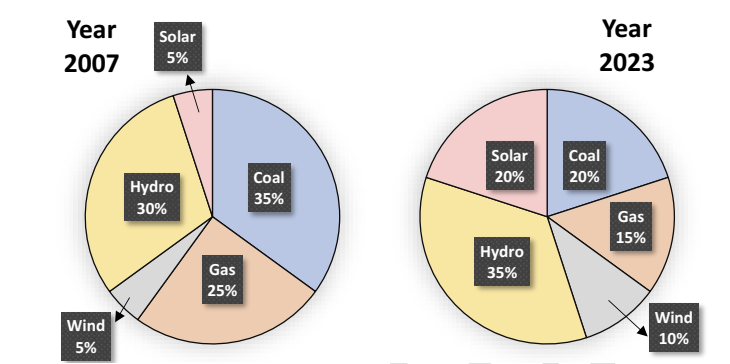
\includegraphics[width=0.5\columnwidth]{figs/ass5_0_q8.png}
    \caption{}
    \label{fig:placeholder}
\end{figure}

The renewable sources of electricity generation consist of Hydro, Solar and Wind. Assuming that the total electricity generated remains the same from 2007 to 2023, what is the percentage increase in the share of the renewable sources of electricity generation over this period?  

\begin{enumerate}
\item 25\%  
\item 50\%  
\item 77.5\%  
\item 62.5\%  
\end{enumerate}
(GATE XE 2024)

\item A cube is to be cut into 8 pieces of equal size and shape. Here, each cut should be straight and it should not stop till it reaches the other end of the cube.  

The minimum number of such cuts required is  

\begin{enumerate}
\item 3  
\item 4  
\item 7  
\item 8  
\end{enumerate}
(GATE XE 2024)

\item In the $4 \times 4$ array shown below, each cell of the first three rows has either a cross (X) or a number.  

$$
\begin{array}{|c|c|c|c|}
\hline
1 & X & 4 & 3 \\ \hline
X & 5 & 5 & 4 \\ \hline
3 & X & 6 & X \\ \hline
  &   &   &   \\ \hline
\end{array}
$$

The number in a cell represents the count of the immediate neighboring cells (left, right, top, bottom, diagonals) NOT having a cross (X). Given that the last row has no crosses (X), the sum of the four numbers to be filled in the last row is  

\begin{enumerate}
\item 11  
\item 10  
\item 12  
\item 9  
\end{enumerate}
(GATE XE 2024)



\newpage

\begin{center}
    {\Large \textbf{ENGINEERING MATHEMATICS (XE - A)}}
\end{center}

\item[] \textbf{Q11 - Q17 carry one mark each.}
\item Let 
$$
f(x) = 
\begin{cases} 
\pi + x, & -\pi \leq x < 0, \\ 
0, & 0 \leq x < \pi,
\end{cases}
$$
with $f(x+2\pi) = f(x)$. If $F(x)$ represents the Fourier series of $f(x)$, then the value of $F\!\left(-\tfrac{\pi}{2}\right) + F(0)$ is  

\begin{enumerate}
\item 0  
\item $\tfrac{\pi}{2}$  
\item $\pi$  
\item $\tfrac{3\pi}{2}$  
\end{enumerate}
(GATE XE 2024)

\item Let $y$ be a non-zero quadratic polynomial satisfying the differential equation  

$$
(2 + x^2)\,\frac{d^2y}{dx^2} + x\,\frac{dy}{dx} - ky = 0,
$$

where $k$ is a real constant. If $y(1) = 1$, then the value of the integral  

$$
\int_{0}^{1} 2y \, dx
$$

is  

\begin{enumerate}
\item $\tfrac{1}{3}$  
\item $\tfrac{2}{3}$  
\item $1$  
\item $\tfrac{4}{3}$  
\end{enumerate}
(GATE XE 2024)

\item There are four cities, namely, $C_1, C_2, C_3$ and $C_4$. The cities are directly connected by four roads as shown in the picture (not included), that is, $C_1$ is connected with $C_2$, $C_2$ is connected with $C_3$, $C_3$ is connected with $C_4$, and $C_4$ is connected with $C_1$.  

The probability of any road getting independently blocked is $\tfrac{1}{3}$.  

Let $E_1$ be the event of travelling from $C_1$ to $C_3$ via $C_2$ and $E_2$ be the event of travelling from $C_1$ to $C_3$ via $C_4$.  

Then, which of the following statements is correct?  

\begin{figure}[H]
    \centering
    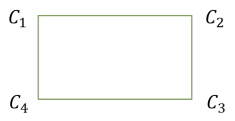
\includegraphics[width=0.5\columnwidth]{figs/ass5_a_q13.png}
    \caption{}
    \label{fig:placeholder}
\end{figure}

\begin{enumerate}
\item $P(E_1 \cup E_2) = \tfrac{56}{81}$  
\item $P(E_1 \cup E_2) = \tfrac{8}{9}$  
\item $P(E_1 \mid E_2) \neq P(E_1) = \tfrac{4}{9}$  
\item $P(E_1 \cap E_2) = 0$   
\end{enumerate}
(GATE XE 2024)

\item Assume that $f:[0,1] \to \mathbb{R}$ is continuous on $[0,1]$ and differentiable on $(0,1)$ such that  
\[
f(x+h) = f(x) + h f'(x+\theta h) \quad \text{for some } 0 < \theta < 1.
\]  
If $f(x) = x^2(1+x)$, and $\theta$ is expressed in terms of $x$ and $h$, then the value of  
$$
\lim_{h \to 0} \theta(x,h)
$$
is  

\begin{enumerate}
\item $\tfrac{1}{3}$ \hfill (GATE XE 2024)  
\item $\tfrac{1}{2}$ \hfill (GATE XE 2024)  
\item $\tfrac{1}{4}$ \hfill (GATE XE 2024)  
\item $\tfrac{4}{5}$ \hfill (GATE XE 2024)  
\end{enumerate}
(GATE XE 2024)

\item Let $A$ be a $3 \times 3$ matrix whose eigenvalues are $2, 3, 4$ and let $I$ be the identity matrix of order $3$. If  
$$
A^{-1} = \frac{1}{2k} (A^2 - 9A) + \frac{13}{k} I
$$
for some integer $k \neq 0$, then the value of $k$ is \_\_\_\_\_  

(GATE XE 2024)

\item For some integer $k$, the differential equation  
$$
x^2 \frac{d^2y}{dx^2} - 3x \frac{dy}{dx} + (k+2)y = 0
$$  
is transformed into  
$$
(D-2)^2 y = 0, \quad \text{where } D = \frac{d}{dt} \text{ and } t = \log x.
$$ 
Then, the value of $k$ is \_\_\_\_\_  

(GATE XE 2024)

\item The approximate value (rounded off to two decimal places) of the integral  
$$
\int_{0}^{\tfrac{1}{2}} e^{-x^2} \, dx,
$$ 
using the Trapezoidal rule with step-size $h = \tfrac{1}{4}$ is \_\_\_\_\_  

(GATE XE 2024)

\item[] \textbf{Q18 - Q21 carry two marks each.} 
\item Consider $f(z)=e^{z}$, where $z=x+iy$ and $i=\sqrt{-1}$. Which of the following
statements is correct?

\begin{enumerate}[label=(\Alph*)]
\item $f$ is periodic.
\item $f$ is not periodic.
\item $\lvert f\rvert=1$.
\item $\arg(f)=y\pm n\pi \text{ for all } n=0,1,2,\ldots$
\end{enumerate}
(GATE XE 2024)

\item Let $P$ and $Q$ be two square matrices of the same order. Then, which of the
following matrices is/are necessarily equal to $(P+2Q)^2$?

\begin{enumerate}[label=(\Alph*)]
\item $P^{2}+4PQ+4Q^{2}$
\item $P(P+2Q)+Q(2P+4Q)$
\item $(P+2Q)(2Q+P)$
\item $P^{2}+2PQ+2QP+4Q^{2}$
\end{enumerate}
(GATE XE 2024)

\item If
$$
\int_{0}^{a}\left(\int_{\sqrt{x/a}}^{\,1} e^{\,y^{3}}\,dy\right)dx \;=\; e-1,\qquad a>0,
$$
then the value (in integer) of $a$ is \_\_\_\_\_.

(GATE XE 2024)

\item Consider the vector field
$
\vec F=(2x+y^{2})\,\hat{\imath}+(2xy+3y)\,\hat{\jmath}
$
and 
$
\alpha_m=\int_{C_m}\vec F\cdot d\vec r,\quad m=1,2,
$
where $C_1$ is an arc of the unit circle connecting the points $(1,0)$ and $(0,1)$ and $C_2$ is the straight line connecting the points $(1,0)$ and $(0,1)$. Then, the value (in integer) of 
$
2\left(\alpha_1^{2}+3\alpha_2^{2}\right)
$
is \_\_\_\_\_\_.

(GATE XE 2024)

\begin{center}
    \textbf{END OF SECTION - A}
\end{center}

\newpage

\begin{center}
    {\Large \textbf{FLUID MECHANICS (XE - B)}}
\end{center}

\item[] \textbf{Q22 - Q30 carry one mark each.}
\item Which one of the following figures shows the \textbf{CORRECT} dependence of apparent viscosity $\eta$ on rate of shear strain $\left(du/dy\right)$ for pseudoplastic (shear-thinning) fluids?

\begin{enumerate}
\item  \begin{figure}[H]
    \centering
    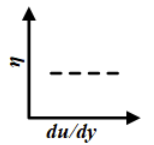
\includegraphics[width=0.3\columnwidth]{figs/ass5_b_q22_a.png}
    \caption{}
    \label{fig:placeholder}
\end{figure}

\item   \begin{figure}[H]
    \centering
    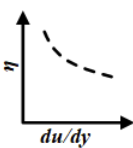
\includegraphics[width=0.3\columnwidth]{figs/ass5_b_q22_b.png}
    \caption{}
    \label{fig:placeholder}
\end{figure}

\item   \begin{figure}[H]
    \centering
    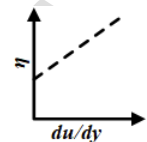
\includegraphics[width=0.3\columnwidth]{figs/ass5_b_q22_c.png}
    \caption{}
    \label{fig:placeholder}
\end{figure}

\item    \begin{figure}[H]
    \centering
    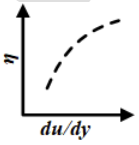
\includegraphics[width=0.3\columnwidth]{figs/ass5_b_q22_d.png}
    \caption{}
    \label{fig:placeholder}
\end{figure}
\end{enumerate}

(GATE XE 2024)

\item The locus of temporary locations of all particles that have passed through a fixed point in the flow field at a particular instant is known as
\begin{enumerate}
\item streamline
\item streakline
\item pathline
\item timeline
\end{enumerate}

(GATE XE 2024)

\item Consider the velocities $u, v,$ and $w$ in $x$-, $y$-, and $z$-directions, respectively. The vorticity expression in the $y$-$z$ plane is
\begin{enumerate}
\item $\dfrac{\partial v}{\partial x}-\dfrac{\partial u}{\partial y}$
\item $\dfrac{\partial v}{\partial y}-\dfrac{\partial w}{\partial z}$
\item $\dfrac{\partial w}{\partial y}-\dfrac{\partial v}{\partial z}$
\item $\dfrac{\partial u}{\partial z}-\dfrac{\partial w}{\partial x}$
\end{enumerate}

(GATE XE 2024)

\item For the laminar, incompressible flow over a flat plate with uniform free stream velocity, the axial pressure gradient within the boundary layer is
\begin{enumerate}
\item greater than zero.
\item less than zero.
\item equal to zero.
\item equal to the axial velocity gradient.
\end{enumerate}

(GATE XE 2024)

\item Let $\vec{r}$, $\vec{V}$, and $m$ be position vector, velocity vector, and mass, respectively in a control mass system. Which one of the following properties is considered as conserved extensive property in Reynolds Transport Theorem to obtain the angular momentum equation?
\begin{enumerate}
\item $\vec{r}\times m\vec{V}$
\item $\vec{r}\times \vec{V}$
\item $m\vec{V}$
\item $m$
\end{enumerate}

(GATE XE 2024)

\item The hydraulic diameter for a circular pipe of radius $R$ is
\begin{enumerate}
\item $0.5R$
\item $R$
\item $2R$
\item $4R$
\end{enumerate}

(GATE XE 2024)

\item For incompressible, laminar, fully developed flow through a circular pipe, Darcy friction factor and Fanning friction factor are represented as $f$ and $c_f$, respectively. Which one of the following options is correct?
\begin{enumerate}
\item $f = 0.25\,c_f$
\item $f = 0.5\,c_f$
\item $f = 2\,c_f$
\item $f = 4\,c_f$
\end{enumerate}

(GATE XE 2024)

\item For an immersed neutrally buoyant body to be in stable equilibrium, the center of gravity of the body is directly
\begin{enumerate}
\item above the metacenter.
\item below the metacenter.
\item above the center of buoyancy.
\item below the center of buoyancy.
\end{enumerate}

(GATE XE 2024)

\item The absolute pressure in a chamber is measured as $400$ mm Hg at a location where the atmospheric pressure is $700$ mm Hg. A vacuum gauge connected to the chamber reads \_\_\_\_\_\_ mm Hg \textit{(answer in integer)}.

(GATE XE 2024)

\item[] \textbf{Q31 - Q43 carry two marks each.}
\item A thin film of an incompressible, Newtonian liquid (density $\rho$, viscosity $\mu$) with an
uniform thickness ($h$) is flowing down on a vertical plate. The flow is driven by gravity ($g$) alone.
Assume zero shear stress condition at the free surface.

\begin{figure}[H]
    \centering
    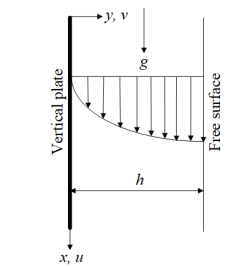
\includegraphics[width=0.5\columnwidth]{figs/ass5_b_q31.png}
    \caption{}
    \label{fig:placeholder}
\end{figure}

The maximum velocity is given by
\begin{enumerate}
\item $\displaystyle \frac{1}{2\mu}\,\rho g h^{2}$
\item $\displaystyle \frac{1}{4\mu}\,\rho g h^{2}$
\item $\displaystyle \frac{1}{\mu}\,\rho g h^{2}$
\item $\displaystyle \frac{1}{8\mu}\,\rho g h^{2}$
\end{enumerate}

(GATE XE 2024)

\item A one-eighth scale model of a car is to be tested in a wind tunnel. If the air velocity
over the car is 16 m/s, what should be the air velocity (in m/s) in the wind tunnel in order
to achieve similarity between the model and the prototype?
\begin{enumerate}
\item 2
\item 16
\item 64
\item 128
\end{enumerate}

(GATE XE 2024)

\item A set of basic dimensions, mass, length, and time are represented by $M$, $L$, and $T$,
respectively. What will be the dimensions of pressure in $M$–$L$–$T$ system?
\begin{enumerate}
\item $M L^{-1} T^{-2}$
\item $M L T^{-2}$
\item $M L T^{-1}$
\item $M L^{-1} T^{-1}$
\end{enumerate}

(GATE XE 2024)

\item Consider a fluid flow around an airfoil as shown in figure. 

\begin{figure}[H]
    \centering
    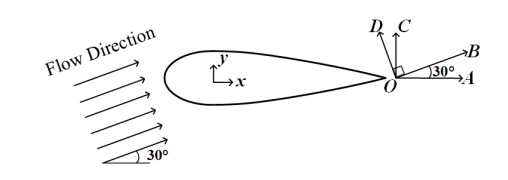
\includegraphics[width=0.5\columnwidth]{figs/ass5_b_q34.png}
    \caption{}
    \label{fig:placeholder}
\end{figure}

The directions of drag force and lift force, respectively are along
\begin{enumerate}
\item OA and OC.
\item OA and OD.
\item OB and OC.
\item OB and OD.
\end{enumerate}

(GATE XE 2024)

\item A vessel which contains a volatile liquid and its vapour is connected with a mercury manometer as shown in the figure. Both the liquid and vapour phases are at equilibrium. The vapour pressure and density of the volatile liquid are $107.6\ \text{kPa}$ and $700\ \text{kg m}^{-3}$, respectively. The density of mercury is $13600\ \text{kg m}^{-3}$. Acceleration due to gravity ($g$) is $10\ \text{m s}^{-2}$ and atmospheric pressure is $101\ \text{kPa}$. Hydrostatic pressure created by the weight of the vapour is neglected.

\begin{figure}[H]
    \centering
    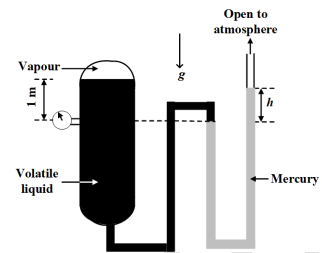
\includegraphics[width=0.5\columnwidth]{figs/ass5_b_q35.png}
    \caption{}
    \label{fig:placeholder}
\end{figure}
The height, $h$ (in m, rounded off to two decimal places) of the mercury column in figure is \_\_\_\_\_\_. 

(GATE XE 2024)

\item The velocity in a one-dimensional flow is given by
$
u(x)=\frac{a}{(b-x)^2}\ \text{m s}^{-1},
$
where $a=8\ \text{m}^3\text{s}^{-1}$ and $b=4\ \text{m}$. The acceleration (in $\text{m s}^{-2}$, answer in integer) at $x=2\ \text{m}$ is \_\_\_\_\_\_\_. 

(GATE XE 2024)

\item Consider two parallel plates separated by a distance of $1\ \text{cm}$ filled with a Newtonian fluid of viscosity $10^{-2}\ \text{Pa}\cdot\text{s}$. The top plate is moving with a velocity of $1\ \text{m s}^{-1}$ whereas the bottom plate is stationary. The shear stress (in Pa, rounded off to one decimal place) on the top plate is \_\_\_\_\_\_\_.

(GATE XE 2024)

\item A circular water jet of diameter $50\ \text{mm}$ impinges with a velocity of $18\ \text{m s}^{-1}$ normal to a plate. The density of water is $1000\ \text{kg m}^{-3}$ and gravity force is neglected.

\begin{figure}[H]
    \centering
    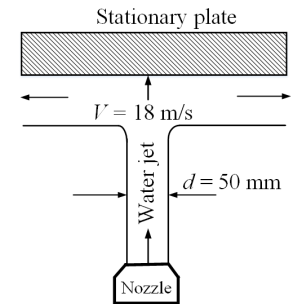
\includegraphics[width=0.5\columnwidth]{figs/ass5_b_q38.png}
    \caption{}
    \label{fig:placeholder}
\end{figure}

The magnitude of net force (in N, \emph{rounded off to two decimal places}) imparted by the jet on the stationary plate is \_\_\_\_\_\_. 

(GATE XE 2024)

\item Consider the steady, incompressible flow of water in a horizontal pipe of constant diameter $1\ \text{m}$ with an inlet velocity of $12\ \text{m s}^{-1}$. 

\begin{figure}[H]
    \centering
    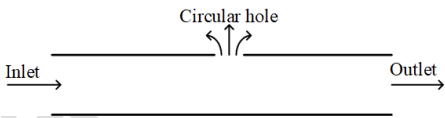
\includegraphics[width=0.5\columnwidth]{figs/ass5_b_q39.png}
    \caption{}
    \label{fig:placeholder}
\end{figure}

As shown in figure, water is lost through a circular hole of diameter $0.6\ \text{m}$ at the rate of $4.53\ \text{m}^3\text{/s}$.
The outlet velocity (in $\text{m s}^{-1}$, \emph{rounded off to two decimal places}) of water in the pipe is \_\_\_\_\_\_. 

(GATE XE 2024)

\item The axial velocity profile of a laminar, incompressible and fully-developed flow in a circular pipe of radius $R$ is given as
$
u_z \;=\; -\,\frac{1}{4\mu}\,\frac{\partial p}{\partial z}\,R^2\left(1-\frac{r^2}{R^2}\right),
$
where $r$, $z$, $\mu$, and $p$ are radial direction, axial direction, fluid viscosity, and pressure, respectively. If the average velocity of the flow is given by
$
u_{z,\mathrm{avg}} \;=\; \frac{1}{K}\left(-\,\frac{R^2}{\mu}\,\frac{\partial p}{\partial z}\right),
$
then the value of $K$ (\emph{answer in integer}) is \_\_\_\_\_. 

(GATE XE 2024)

\item The velocity potential function in a two-dimensional flow field is given by  
$
\phi(x,y)=-(a\,xy+b\,x^{2}-b\,y^{2})\ \text{m}^2/\text{s},
$
where $a=2\ \text{s}^{-1}$ and $b=0.5\ \text{s}^{-1}$. The magnitude of the velocity (in m/s, answer in integer) at $x=2\ \text{m}, y=1\ \text{m}$ is \_\_\_\_\_\_\_.  

(GATE XE 2024)

\item Consider the incompressible, steady and irrotational flow through a concentric reducer in a horizontal pipeline. The pipe diameter reduces from $d_1=12\ \text{cm}$ to $d_2=4\ \text{cm}$. The pressure at position 1 and position 2 of the reducer is $p_1=55\ \text{kPa}$ and $p_2=27\ \text{kPa}$, respectively. The specific weight of the fluid is $7\ \text{kN/m}^3$. Acceleration due to gravity is $10\ \text{m/s}^2$.

\begin{figure}[H]
    \centering
    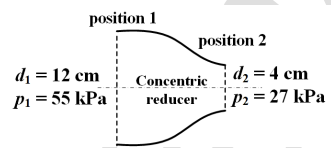
\includegraphics[width=0.5\columnwidth]{figs/ass5_b_q42.png}
    \caption{}
    \label{fig:placeholder}
\end{figure}

Neglecting frictional effects, the mass flow rate (in kg/s, rounded off to two decimal places) of the fluid through the reducer is \_\_\_\_\_\_.  

(GATE XE 2024)

\item Consider the incompressible fluid flow over a flat plate with a free stream velocity $U_\infty = 1\ \text{m/s}$. The fluid kinematic viscosity is $10^{-6}\ \text{m}^2/\text{s}$ and density is $1\ \text{kg/m}^3$. The velocity profile within the boundary layer at any location $x$ is given by  
$
u(y)=U_\infty\left(\frac{3y}{2\delta} - \frac{1}{2}\frac{y^{3}}{\delta^{3}}\right),
$
where the boundary-layer thickness is  
$
\delta = \frac{4.64\,x}{\sqrt{\mathrm{Re}_x}}, \quad \mathrm{Re}_x = \frac{U_\infty\,x}{\nu}.
$
The local wall shear stress at $x=1\ \mathrm{m}$ from the leading edge is \_\_\_\_\_\_ $\times 10^{-3}\ \mathrm{N/m}^2$ (rounded off to two decimal places).  

(GATE XE 2024)

\begin{center}
    \textbf{END OF SECTION - B}
\end{center}

\newpage

\begin{center}
    {\Large \textbf{MATERIALS SCIENCE (XE - C)}}
\end{center}

\item[] \textbf{Q44 - Q52 carry one mark each.}
\item The correct combination of phases in the one-component H$_2$O phase diagram (schematic not shown) is
\begin{figure}[H]
    \centering
    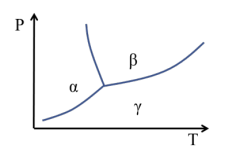
\includegraphics[width=0.5\columnwidth]{figs/ass5_c_q44.png}
    \caption{}
    \label{fig:placeholder}
\end{figure}

\begin{enumerate}
\item $\alpha$ -- water; $\beta$ -- vapour; $\gamma$ -- ice
\item $\alpha$ -- ice; $\beta$ -- water; $\gamma$ -- vapour
\item $\alpha$ -- vapour; $\beta$ -- ice; $\gamma$ -- water
\item $\alpha$ -- water; $\beta$ -- ice; $\gamma$ -- vapour
\end{enumerate}
(GATE XE 2024)

\item Mechanical behaviour of a crystalline ceramic material is best described as
\begin{enumerate}
\item ductile
\item brittle
\item viscoelastic
\item viscoplastic
\end{enumerate}
(GATE XE 2024)

\item Differential scanning calorimetry involves measurement of
\begin{enumerate}
\item weight change
\item entropy
\item heat
\item vapour pressure
\end{enumerate}
(GATE XE 2024)

\item In ball milling of ceramic powder, selection of grinding media depends on the \_\_\_\_\_\_ difference between grinding media and powder particles.
\begin{enumerate}
\item thermal conductivity
\item dielectric constant
\item hardness
\item density
\end{enumerate}
(GATE XE 2024)

\item Which one of the following unit cell parameters represents a tetragonal crystal system?
\begin{enumerate}
\item $a = b = c \ ; \ \alpha = \beta = \gamma \neq 90^\circ$
\item $a \neq b \neq c \ ; \ \alpha = \beta = \gamma = 90^\circ$
\item $a = b \neq c \ ; \ \alpha = \beta = 90^\circ, \ \gamma = 120^\circ$
\item $a = b \neq c \ ; \ \alpha = \beta = \gamma = 90^\circ$
\end{enumerate}
(GATE XE 2024)

\item Which of the following types of materials exhibit(s) positive magnetic susceptibility?
\begin{enumerate}
\item Paramagnetic
\item Diamagnetic
\item Ferrimagnetic
\item Ferromagnetic
\end{enumerate}
(GATE XE 2024)

\item Which of the following is/are responsible for pitting corrosion in a metal?
\begin{enumerate}
\item Rough surface
\item Grain boundaries
\item Polished surface
\item Polymer coated metal surface
\end{enumerate}
(GATE XE 2024)

\item In thermogravimetric analysis (TGA), weight change of a material sample during decomposition with temperature is shown in the figure below. $W_i$ and $W_f$ represent the weight of the material, corresponding to temperatures $T_i$ and $T_f$, respectively. Which of the following factor(s) can influence $T_i$ and $T_f$?

\begin{figure}[H]
    \centering
    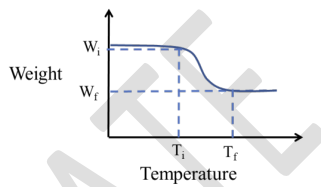
\includegraphics[width=0.5\columnwidth]{figs/ass5_c_q51.png}
    \caption{}
    \label{fig:placeholder}
\end{figure}
\begin{enumerate}
\item Heating rate
\item Particle size of the material
\item Atmosphere in the sample chamber
\item Initial weight of the sample
\end{enumerate}
(GATE XE 2024)

\item The work done by a body expanding from an initial state $A$ to the final state $B$, as shown in the $P$--$V$ diagram below, is (in units of litre$\,$--$\,$atm, rounded off to nearest integer) \_\_\_\_\_\_. 

\begin{figure}[H]
    \centering
    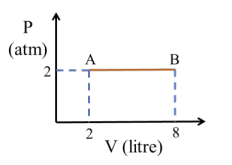
\includegraphics[width=0.5\columnwidth]{figs/ass5_c_q52.png}
    \caption{}
    \label{fig:placeholder}
\end{figure}

(GATE XE 2024)

\item[] \textbf{Q53 - Q65 carry two marks each.}
\item A binary phase diagram is given below.

\begin{figure}[H]
    \centering
    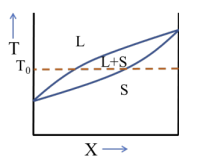
\includegraphics[width=0.5\columnwidth]{figs/ass5_c_q53.png}
    \caption{}
    \label{fig:placeholder}
\end{figure}

Which one of the following figures qualitatively represents the $G$--$X$ (Gibbs free energy -- composition) plot at temperature $T_0$ shown in the phase diagram?

\begin{enumerate}
\item \begin{figure}[H]
    \centering
    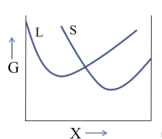
\includegraphics[width=0.5\columnwidth]{figs/ass5_c_q53_a.png}
    \caption{}
    \label{fig:placeholder}
\end{figure}
\item \begin{figure}[H]
    \centering
    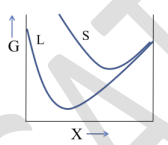
\includegraphics[width=0.5\columnwidth]{figs/ass5_c_q53_b.png}
    \caption{}
    \label{fig:placeholder}
\end{figure}
\item \begin{figure}[H]
    \centering
    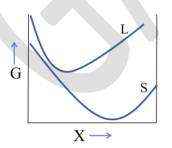
\includegraphics[width=0.5\columnwidth]{figs/ass5_c_q53_c.png}
    \caption{}
    \label{fig:placeholder}
\end{figure}
\item \begin{figure}[H]
    \centering
    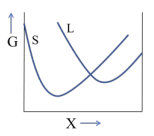
\includegraphics[width=0.5\columnwidth]{figs/ass5_c_q53_d.png}
    \caption{}
    \label{fig:placeholder}
\end{figure}
\end{enumerate}

(GATE XE 2024)

\item Which one of the following figures corresponds to the density of states $g(E)$ of a typical intrinsic semiconductor?
($E$ represents the energy level of a charge carrier)

\begin{enumerate}
\item \begin{figure}[H]
    \centering
    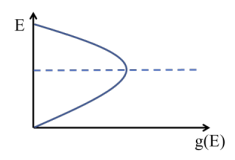
\includegraphics[width=0.5\columnwidth]{figs/ass5_c_q54_a.png}
    \caption{}
    \label{fig:placeholder}
\end{figure}
\item \begin{figure}[H]
    \centering
    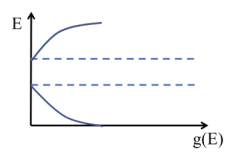
\includegraphics[width=0.5\columnwidth]{figs/ass5_c_q54_b.png}
    \caption{}
    \label{fig:placeholder}
\end{figure}
\item \begin{figure}[H]
    \centering
    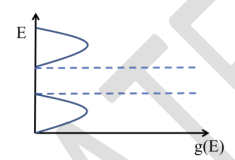
\includegraphics[width=0.5\columnwidth]{figs/ass5_c_q54_c.png}
    \caption{}
    \label{fig:placeholder}
\end{figure}
\item \begin{figure}[H]
    \centering
    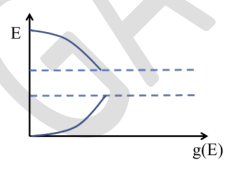
\includegraphics[width=0.5\columnwidth]{figs/ass5_c_q54_d.png}
    \caption{}
    \label{fig:placeholder}
\end{figure}
\end{enumerate}

(GATE XE 2024)

\item The Miller indices for the shaded plane shown in the unit cell below is

\begin{figure}[H]
    \centering
    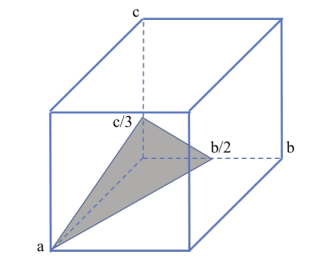
\includegraphics[width=0.5\columnwidth]{figs/ass5_c_q55.png}
    \caption{}
    \label{fig:placeholder}
\end{figure}

\begin{enumerate}
\item $[632]$
\item $[123]$
\item $(632)$
\item $(123)$
\end{enumerate}

(GATE XE 2024)

\item Which one of the following curves best represents the $E$ vs. $f(E)$ behavior of the hot end of a metal rod demonstrating Seebeck Effect? ($f(E)$ is the probability of electron occupancy at an energy state $E$; $E_F$ is the Fermi energy)

\begin{enumerate}
\item \begin{figure}[H]
    \centering
    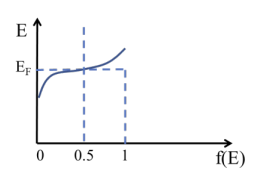
\includegraphics[width=0.5\columnwidth]{figs/ass5_c_q56_a.png}
    \caption{}
    \label{fig:placeholder}
\end{figure}
\item \begin{figure}[H]
    \centering
    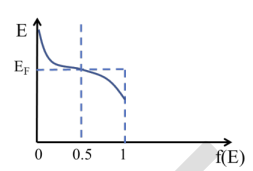
\includegraphics[width=0.5\columnwidth]{figs/ass5_c_q56_b.png}
    \caption{}
    \label{fig:placeholder}
\end{figure}
\item \begin{figure}[H]
    \centering
    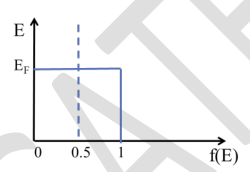
\includegraphics[width=0.5\columnwidth]{figs/ass5_c_q56_c.png}
    \caption{}
    \label{fig:placeholder}
\end{figure}
\item \begin{figure}[H]
    \centering
    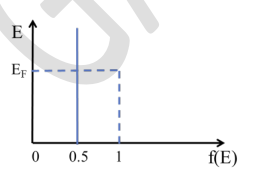
\includegraphics[width=0.5\columnwidth]{figs/ass5_c_q56_d.png}
    \caption{}
    \label{fig:placeholder}
\end{figure}
\end{enumerate}

(GATE XE 2024)

\item In a typical light emitting diode (LED), which of the following type(s) of materials is/are used?

\begin{enumerate}
\item Indirect bandgap semiconductor with transition metal impurities
\item Direct bandgap semiconductor
\item Indirect bandgap semiconductor with isoelectronic impurities
\item Indirect bandgap semiconductor without any impurity
\end{enumerate}

(GATE XE 2024)

\item Which of the following options is/are true for glass transition temperature $T_g$?

\begin{enumerate}
\item Above $T_g$, glass transforms from an amorphous solid to a viscous liquid.
\item At $T_g$, glass transforms from an amorphous solid to a crystalline solid.
\item $T_g$ is dependent on the heating rate.
\item Below $T_g$, nucleation and growth takes place in glass.
\end{enumerate}

(GATE XE 2024)

\item Which of the following figures schematically represent(s) either the Frenkel defect or the Schottky defect in ionic solids?

\begin{enumerate}
\item \begin{figure}[H]
    \centering
    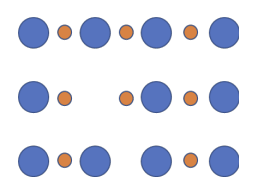
\includegraphics[width=0.5\columnwidth]{figs/ass5_c_q59_a.png}
    \caption{}
    \label{fig:placeholder}
\end{figure}
\item \begin{figure}[H]
    \centering
    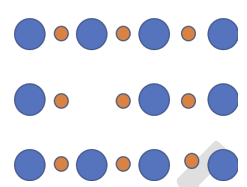
\includegraphics[width=0.5\columnwidth]{figs/ass5_c_q59_b.png}
    \caption{}
    \label{fig:placeholder}
\end{figure}
\item \begin{figure}[H]
    \centering
    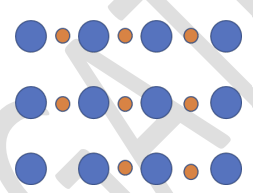
\includegraphics[width=0.5\columnwidth]{figs/ass5_c_q59_c.png}
    \caption{}
    \label{fig:placeholder}
\end{figure}
\item \begin{figure}[H]
    \centering
    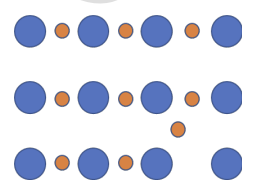
\includegraphics[width=0.5\columnwidth]{figs/ass5_c_q59_d.png}
    \caption{}
    \label{fig:placeholder}
\end{figure}
\end{enumerate}

(GATE XE 2024)

\item Given that $k$ is the first-order reaction rate constant and $T$ is the temperature on an absolute scale, the temperature dependence of the rate constant is/are represented by

\begin{enumerate}
\item \begin{figure}[H]
    \centering
    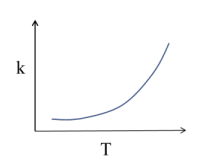
\includegraphics[width=0.5\columnwidth]{figs/ass5_c_q60_a.png}
    \caption{}
    \label{fig:placeholder}
\end{figure}
\item \begin{figure}[H]
    \centering
    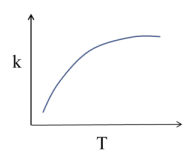
\includegraphics[width=0.5\columnwidth]{figs/ass5_c_q60_b.png}
    \caption{}
    \label{fig:placeholder}
\end{figure}
\item \begin{figure}[H]
    \centering
    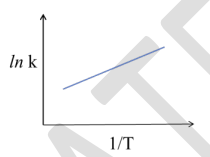
\includegraphics[width=0.5\columnwidth]{figs/ass5_c_q60_c.png}
    \caption{}
    \label{fig:placeholder}
\end{figure}
\item \begin{figure}[H]
    \centering
    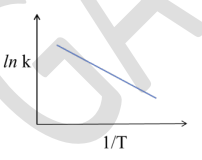
\includegraphics[width=0.5\columnwidth]{figs/ass5_c_q60_d.png}
    \caption{}
    \label{fig:placeholder}
\end{figure}
\end{enumerate}

(GATE XE 2024)

\item For chemical vapour deposition (CVD) process, which of the following statements is/are correct?

\begin{enumerate}
\item Target material is stripped off by the bombardment of positive ions.
\item Source material is vapourized and thermally decomposed.
\item Partial hydrolysis of alkoxide in water solvent.
\item Suitable for preparing films of high density and uniform thickness.
\end{enumerate}

(GATE XE 2024)

\item At room temperature, the electrical conductivity and electron mobility for aluminium are $3.8\times 10^{7}\;(\Omega\,\text{m})^{-1}$ and $0.0012\;\text{m}^2(\text{V}\,\text{s})^{-1}$, respectively. Density of free electrons for aluminium at room temperature is (in units of $\text{m}^{-3}$) \_\_\_\_\_ $\times 10^{27}$ (rounded off to nearest integer).

Given: Electrical charge on an electron is $1.6\times 10^{-19}\ \text{C}$.

(GATE XE 2024)

\item A $2\ \text{mm}$ thick palladium sheet of $1000\ \text{mm}^2$ cross section is used as a diffusional membrane to purify hydrogen. The hydrogen concentration is maintained at a steady state with $c_h=1.5\ \text{kg m}^{-3}$ and $c_l=0.3\ \text{kg m}^{-3}$ on the two sides of the membrane. 
\begin{figure}[H]
    \centering
    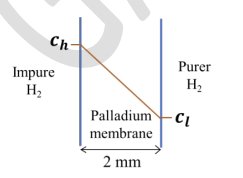
\includegraphics[width=0.5\columnwidth]{figs/ass5_c_q63.png}
    \caption{}
    \label{fig:placeholder}
\end{figure}


The rate of hydrogen purification is (in units of $\text{kg hr}^{-1}$) \_\_\_\_\_\_ $\times 10^{-6}$ (rounded off to one decimal place).

Given: The diffusion coefficient of hydrogen in palladium is $1.0\times 10^{-8}\ \text{m}^2\text{s}^{-1}$.

(GATE XE 2024)

\item In X-ray powder diffraction pattern obtained from a face centered cubic (FCC) metal, the first five reflections are at $\theta = 21.65^\circ,\ 25.21^\circ,\ 37.06^\circ,\ x^\circ,$ and $47.58^\circ$. The Bragg angle of the fourth reflection is missed out and is represented by $x$. The value of $x$ (in degree) is \_\_\_\_\_\_ (rounded off to one decimal place).

(GATE XE 2024)

\item Consider a unidirectionally aligned continuous glass fibre reinforced epoxy composite with $40$ vol.\% reinforcement. The elastic modulus of the composite along the fibre direction is (in units of GPa) \_\_\_\_\_\_ (rounded off to one decimal place).

Given: Elastic modulus of epoxy is $6.9$ GPa and that of glass fibre is $69$ GPa.

(GATE XE 2024)

\begin{center}
    \textbf{END OF SECTION - C}
\end{center}

\newpage

\begin{center}
    {\Large \textbf{SOLID MECHANICS (XE - D)}}
\end{center}

\item[] \textbf{Q66 - Q74 carry one mark each.}
\item The engineering stress $(\sigma)$ vs.\ engineering strain $(\varepsilon)$ curve obtained by conducting a uniaxial tension test on a steel specimen is shown (sketch not to scale). The specimen exhibits cup-and-cone failure within its gage length. Which point on the curve corresponds to the beginning of \emph{necking} in the test specimen?

\begin{figure}[H]
    \centering
    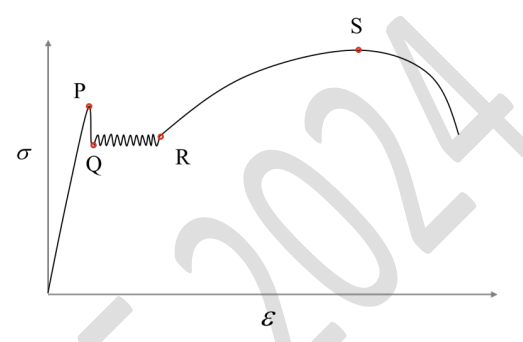
\includegraphics[width=0.5\columnwidth]{figs/ass5_d_q66.png}
    \caption{}
    \label{fig:placeholder}
\end{figure}

\begin{enumerate}
\item P
\item Q
\item R
\item S
\end{enumerate}

(GATE XE 2024)

\item An L-shaped rigid member is fixed at the midpoint of a simply-supported beam, as shown in figure (i). The member is subjected to a vertically downward force $P$ at its free end. In an equivalent system, the member along with the applied load is replaced with a force $Q=P$ and a moment $M$ (see figure (ii)). Which of the following statements is correct?

(Neglect the mass of the beam and of the rigid member.)

\begin{figure}[H]
    \centering
    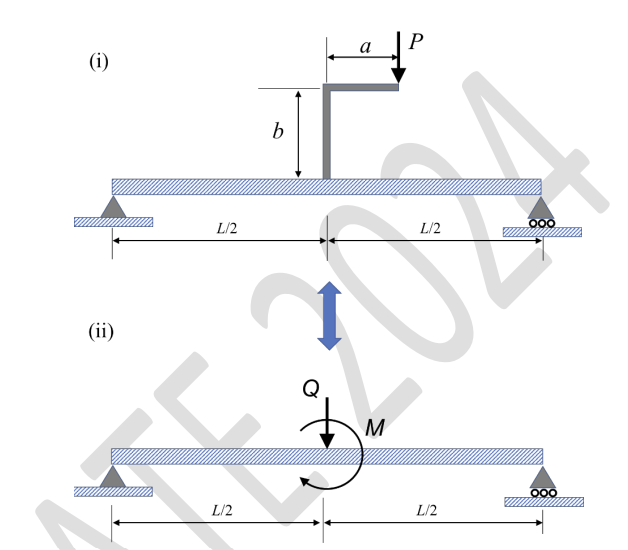
\includegraphics[width=0.5\columnwidth]{figs/ass5_d_q67.png}
    \caption{}
    \label{fig:placeholder}
\end{figure}

\begin{enumerate}
\item $M = P a$
\item $M = P b$
\item $M = P(a+b)$
\item $M = 0$
\end{enumerate}

(GATE XE 2024)

\item A block of weight $W$, placed on a surface, is subjected to a horizontal force $P$ as shown in the figure. The line of action of force $P$ passes through the center-of-gravity of the block. The magnitude of $P$ is such that the block remains at rest. If $N$ is the resultant normal reaction exerted by the surface, and $F$ is the frictional force acting on the bottom surface of the block, then which of the following represents the correct free body diagram of the block?

\begin{figure}[H]
    \centering
    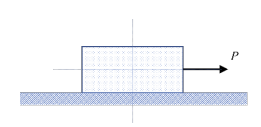
\includegraphics[width=0.5\columnwidth]{figs/ass5_d_q68.png}
    \caption{}
    \label{fig:placeholder}
\end{figure}

\begin{enumerate}
\item \begin{figure}[H]
    \centering
    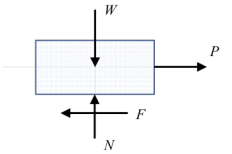
\includegraphics[width=0.5\columnwidth]{figs/ass5_d_q68_a.png}
    \caption{}
    \label{fig:placeholder}
\end{figure}
\item \begin{figure}[H]
    \centering
    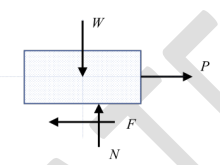
\includegraphics[width=0.5\columnwidth]{figs/ass5_d_q68_b.png}
    \caption{}
    \label{fig:placeholder}
\end{figure}
\item \begin{figure}[H]
    \centering
    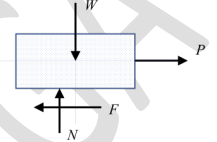
\includegraphics[width=0.5\columnwidth]{figs/ass5_d_q68_c.png}
    \caption{}
    \label{fig:placeholder}
\end{figure}
\item \begin{figure}[H]
    \centering
    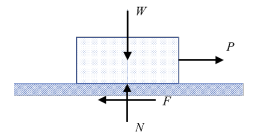
\includegraphics[width=0.5\columnwidth]{figs/ass5_d_q68_d.png}
    \caption{}
    \label{fig:placeholder}
\end{figure}
\end{enumerate}

(GATE XE 2024)

\item A mass $M$ is hung from a frictionless, massless pulley. The pulley is suspended by using an inextensible, massless rope of which one end is directly fixed to a support, and the other end is connected to the support through a linear spring of stiffness constant $k$ (see figure). The natural frequency of this system is

\begin{figure}[H]
    \centering
    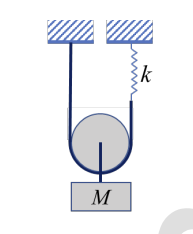
\includegraphics[width=0.5\columnwidth]{figs/ass5_d_q69.png}
    \caption{}
    \label{fig:placeholder}
\end{figure}

\begin{enumerate}
\item $\sqrt{\dfrac{4k}{M}}$
\item $\sqrt{\dfrac{2k}{M}}$
\item $\sqrt{\dfrac{k}{M}}$
\item $\sqrt{\dfrac{k}{2M}}$
\end{enumerate}

(GATE XE 2024)

\item A simply-supported beam of rectangular cross-section (width $w$ and height $h$) is subjected to the loads as shown in the figure (i). The enlarged view of the beam cross-section is shown in figure (ii). The coordinate system is indicated in the figures. Assuming Euler-Bernoulli beam approximation, the shear stress $\tau_{xz}$ and normal stress $\sigma_{xx}$ at the origin, $O$ are respectively given by

\begin{figure}[H]
    \centering
    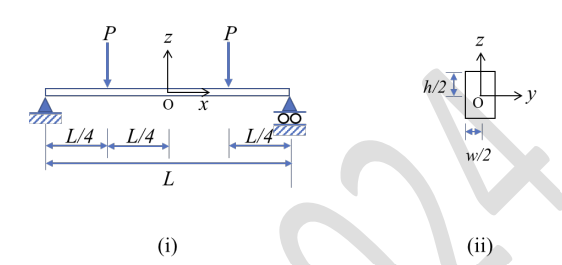
\includegraphics[width=0.5\columnwidth]{figs/ass5_d_q70.png}
    \caption{}
    \label{fig:placeholder}
\end{figure}

\begin{enumerate}
\item $\dfrac{3P}{2wh}, \ \dfrac{3PL}{2wh^2}$
\item $0, \ \dfrac{3PL}{2wh^2}$
\item $\dfrac{3P}{2wh}, \ 0$
\item $0, \ 0$
\end{enumerate}

(GATE XE 2024)

\item An ice-skater starts spinning during her performance. As she retracts her arms and legs closer to her body, her angular velocity \_\_\_\_\_\_\_\_\_\_\_\_\_\_\_\_\_\_

\begin{enumerate}
\item increases
\item decreases
\item remains the same
\item goes to zero
\end{enumerate}

(GATE XE 2024)

\item A solid circular shaft of diameter 100 mm is subjected to a torque $3\pi$ kNm. Which of the following statements about the state of stress in the shaft is/are correct?

\begin{enumerate}
\item The maximum shear stress is 48 MPa
\item The maximum tensile stress is 48 MPa
\item The magnitude of maximum compressive stress is 48 MPa
\item The magnitude of shear stress is 48 MPa at all points in the shaft
\end{enumerate}

(GATE XE 2024)

\item A spring is connected to an elastic bar as shown in the figure. The spring has a stiffness constant of $10^7$ N/m. The bar is 70 mm long, and has an area of cross-section $10$ mm$^2$. The Young’s modulus of the bar material is 70,000 MPa. A force $F = 5000$ N is applied at point O along the axis of the bar and the spring. The resulting deflection of Point O in mm (rounded to one decimal place) is \_\_\_\_\_\_\_\_

\begin{figure}[H]
    \centering
    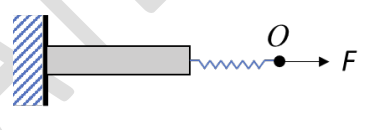
\includegraphics[width=0.5\columnwidth]{figs/ass5_d_q73.png}
    \caption{}
    \label{fig:placeholder}
\end{figure}

(GATE XE 2024)

\item A particle of mass 1 kg is attached to one end of a spring having stiffness of 125 N/m. The free length of the spring is 100 mm. The system is rotated about the other end of the spring at a uniform angular velocity of 5 rad/s. Ignore gravity and consider that the elongation of the spring may be comparable to the free length of the spring. The elongation of the spring (in mm, rounded off to the nearest integer) is \_\_\_\_\_\_\_\_

(GATE XE 2024)

\item[] \textbf{Q75 - Q87 carry two marks each.}

\item A 0-45-90 strain gauge rosette is mounted on an aircraft wing. The co-ordinate system is placed such that the strain gauges p, q and r are oriented at angles $0^\circ$, $45^\circ$ and $90^\circ$, respectively, from the x axis (see figure). The strain readings associated to p, q and r are denoted by $\varepsilon_p$, $\varepsilon_q$, and $\varepsilon_r$, respectively. While conducting a test the strain gauges show the following readings.  

$
\varepsilon_p = 150 \times 10^{-6}, \quad \varepsilon_q = 180 \times 10^{-6}, \quad \varepsilon_r = -90 \times 10^{-6}
$

The developed engineering shear strain $\gamma_{xy}$ associated to the strain gauge data is

\begin{figure}[H]
    \centering
    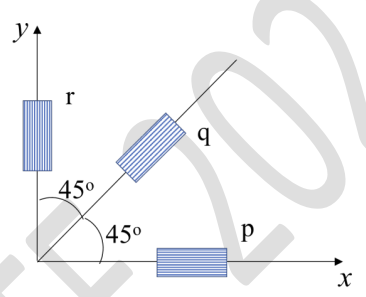
\includegraphics[width=0.5\columnwidth]{figs/ass5_d_q75.png}
    \caption{}
    \label{fig:placeholder}
\end{figure}

\begin{enumerate}
\item $120 \times 10^{-6}$
\item $180 \times 10^{-6}$
\item $300 \times 10^{-6}$
\item $240 \times 10^{-6}$
\end{enumerate}

(GATE XE 2024)

\item A rigid bar PQR is hinged at its end P. As shown in the figure, the bar is pin-connected through two identical links QS and RT at points Q and R, respectively. The other ends of the links, S and T, are fixed. Both links are made of the same material. If the temperature of the links is uniformly increased by $\Delta T$, then which one of the following statements is correct? (Neglect the weight of the rigid bar)

\begin{figure}[H]
    \centering
    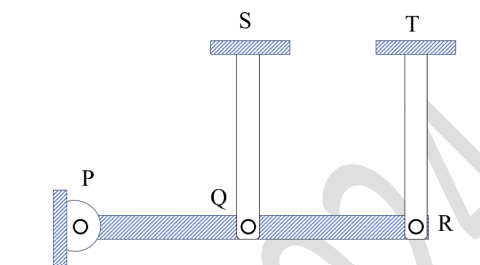
\includegraphics[width=0.5\columnwidth]{figs/ass5_d_q76.png}
    \caption{}
    \label{fig:placeholder}
\end{figure}

\begin{enumerate}
\item Both QS and RT will be stress free.
\item Both QS and RT will be under tension.
\item Both QS and RT will be under compression.
\item QS will be under compression and RT will be under tension.
\end{enumerate}

(GATE XE 2024)

\item A pin-jointed truss has a pin support at the point E and a roller support at the point F. A horizontal force $P$ is applied at pin H as shown in the figure. Which one of the members is in compression?

\begin{figure}[H]
    \centering
    \includegraphics[width=0.5\columnwidth]{figs/IMG_20250823_190304.jpg}
    \caption{}
    \label{fig:placeholder}
\end{figure}

\begin{enumerate}
\item EF
\item FG
\item EG
\item EH
\end{enumerate}

(GATE XE 2024)

\item Two identical rigid slender bars of length $2L$ and mass $m$ are acted upon by a transverse force $F$ at one of te ends as shown in the figure. In the first case, the bar is pinned at the other end. In the second case, the bar is pinned at its mid-point. What should be the magnitude of the force $F$ such that the resulting angular accelerations of the two bars are equal?

\begin{figure}[H]
    \centering
    \includegraphics[width=0.5\columnwidth]{figs/ass5_d_q78.jpg}
    \caption{}
    \label{fig:placeholder}
\end{figure}

\begin{enumerate}
\item $mg$
\item $\dfrac{mg}{2}$
\item $\dfrac{mg}{4}$
\item $\dfrac{mg}{6}$
\end{enumerate}

(GATE XE 2024)

\item A critical point on a component is subjected to the state of stress $[\sigma]$ as given in the following. The yield strength of the material is 400 MPa. By considering maximum shear stress (Tresca) theory, the possible value(s) of $\sigma_0$ at the onset of yielding is/are,

$$
[\sigma] = \myvec{280 & 0 & 0 \\ 0 & \sigma_0 & 0 \\ 0 & 0 & -60} \ \text{MPa}
$$

\begin{enumerate}
\item $340$
\item $680$
\item $-120$
\item $-460$
\end{enumerate}

(GATE XE 2024)

\item A plane passing through a point Q inside a body is shown. The unit normal of the plane is $\hat{n} = 0.6 \hat{i} + 0.8 \hat{j}$, as shown in the figure. The traction (stress) vector on the plane at point Q is given by $\vec{t} = (50 \hat{i} + 20 \hat{j})$ MPa. Given that at point Q, $\sigma_{xx} = \sigma_{yy}$, the shear stress component $\tau_{xy}$ (in MPa, rounded off to two decimal places) is \_\_\_\_\_.

\begin{figure}[H]
    \centering
    \includegraphics[width=0.5\columnwidth]{figs/ass5_d_q80.jpg}
    \caption{}
    \label{fig:placeholder}
\end{figure}

(GATE XE 2024)

\item A rigid massless bar PQR is hinged at its end P and supported through a spring of stiffness $k$ at point Q. A vertically downward force $W=560\ \text{N}$ is applied at the free end R of the bar. If the vertical component of the displacement at R is $30\ \text{mm}$, then the stiffness of the spring (in kN/m, rounded off to one decimal place) is \_\_\_\_\_\_.

\begin{figure}[H]
    \centering
    \includegraphics[width=0.5\columnwidth]{figs/ass5_d_q81.jpg}
    \caption{}
    \label{fig:placeholder}
\end{figure}

(GATE XE 2024)

\item A beam of rectangular cross-section, as shown in the figure, is made of two perfectly bonded layers of different materials and equal thickness. The Young’s moduli of the two materials are $E_1$ and $E_2$, where $E_1 = 2E_2$. The beam is subjected to pure bending. If $t=1\ \text{mm}$, the distance of the neutral plane from the top surface of the beam is \_\_\_\_\_\_ (in mm, rounded off to two decimal places).

\begin{figure}[H]
    \centering
    \includegraphics[width=0.5\columnwidth]{figs/ass5_d_q82.jpg}
    \caption{}
    \label{fig:placeholder}
\end{figure}

(GATE XE 2024)

\item A stepped beam is made of a material whose Young’s modulus is $E$. The dimensions of the two stepped sections are such that the sectional moments of inertia, $I_1$ and $I_2$, are related as $I_1 = 8 I_2$. The beam is fixed at one end and a load of $F$ is applied at the free end as shown in the figure. Under this loading condition, if the strain energy of the stepped beam is written as 
$$U = \beta \frac{F^2 L^3}{E I_1},$$
then the value of $\beta$ is \_\_\_\_\_\_\_ (rounded off to two decimal places).

\begin{figure}[H]
    \centering
    \includegraphics[width=0.5\columnwidth]{figs/ass5_d_q83.png}
    \caption{}
    \label{fig:placeholder}
\end{figure}

(GATE XE 2024)

\item A cylindrical pressure vessel is constructed by bolting two symmetric halves of flanged semi-cylindrical shells. A cross-sectional view of the vessel is shown in the figure. The inner diameter of the vessel is $2\ \text{m}$ and the length is $10\ \text{m}$. Each row comprises $100$ bolts along the length of the vessel. If the vessel is pressurized to a net pressure of $6 \times 10^5\ \text{N/m}^2$, and assuming the end caps of the vessel do not take any load in the radial direction, then the load borne by each bolt is \_\_\_\_\_\_ (in kN, rounded off to one decimal place).

\begin{figure}[H]
    \centering
    \includegraphics[width=0.5\columnwidth]{figs/ass5_d_q84.png}
    \caption{}
    \label{fig:placeholder}
\end{figure}

(GATE XE 2024)

\item A turn-table is rotating about its center with an angular velocity of $2 \ \text{rad/s}$ in the counter-clockwise direction. There is a groove in the turn-table within which a marble moves with a constant speed $v \ \text{m/s}$ relative to the turn-table. At a given instant, the marble is at a radial distance of $1 \ \text{m}$ from the center and the line joining the center of the turn-table with the marble makes an angle of $30^\circ$ with the groove. The value of $v$ (in m/s, rounded off to one decimal place) for which there is no radial acceleration for the marble at this instant is \_\_\_\_\_\_\_\_.

\begin{figure}[H]
    \centering
    \includegraphics[width=0.5\columnwidth]{figs/ass5_d_q85.png}
    \caption{}
    \label{fig:placeholder}
\end{figure}

(GATE XE 2024)

\item The system shown in the figure is in static equilibrium. The spring is massless and has a spring constant of $K = 1 \ \text{kN/m}$. The free length of the spring is $1 \ \text{m}$. All bodies in the system except the spring are rigid and have mass of $M = 1 \ \text{kg}$. All surfaces are frictionless and pin joints are ideal. The elongation of the spring (in mm, rounded off to nearest integer) in this configuration is \_\_\_\_\_\_\_. Take the acceleration due to gravity $g = 10 \ \text{m/s}^2$.

\begin{figure}[H]
    \centering
    \includegraphics[width=0.5\columnwidth]{figs/ass5_d_q86.png}
    \caption{}
    \label{fig:placeholder}
\end{figure}

(GATE XE 2024)

\item A square block of side $1 \ \text{m}$ and mass $10 \ \text{kg}$ is resting on a horizontal surface. The coefficient of static friction between the block and the surface is $0.75$. A horizontal force $P$ acts on the block as shown in the figure. The force $P$ is gradually increased from zero until the block either slides or topples. The maximum value of $h$ (in m, rounded off to two decimal places) for which the block slides without toppling is \_\_\_\_\_\_\_. Take the acceleration due to gravity $g = 10 \ \text{m/s}^2$.

\begin{figure}[H]
    \centering
    \includegraphics[width=0.5\columnwidth]{figs/ass5_d_q87.png}
    \caption{}
    \label{fig:placeholder}
\end{figure}

(GATE XE 2024)

\begin{center}
    \textbf{END OF SECTION - D}
\end{center}

\newpage

\begin{center}
    {\Large \textbf{THERMODYNAMICS (XE - E)}}
\end{center}

\item[] \textbf{Q88 - Q96 carry one mark each.}
\item A heat source at temperature $T_H$ transfers the \textit{same} amount of heat to a sink under the following situations:

\textbf{Case A:} Sink is at temperature $T_{L,1}$  

\textbf{Case B:} Sink is at temperature $T_{L,2}$  

If $T_{L,1} < T_{L,2}$, which one of the following statements is TRUE?

\begin{enumerate}
\item The reversibility is the same, and the entropy generation is greater than zero for Cases A and B  
\item Case B is less reversible with the entropy generation greater than zero  
\item Case B is more reversible with the entropy generation greater than zero  
\item Case B is more reversible with the entropy generation equal to zero  
\end{enumerate}

(GATE XE 2024)

\item Given $v$ is the molar specific volume, $P$ is the pressure, $T$ is the temperature, $R$ is the Universal gas constant, and $a, b$ are van der Waal’s constants.  

The van der Waal’s equation of state is  

$$ P = \frac{RT}{v-b} - \frac{a}{v^2} $$  

The value of  
$$ \left(\frac{\partial v}{\partial T}\right)_{P} \left(\frac{\partial P}{\partial v}\right)_{T} \left(\frac{\partial T}{\partial P}\right)_{v} $$  
is  

\begin{enumerate}
\item $\dfrac{a}{b^2}$  
\item $-1$  
\item $1$  
\item $\dfrac{b^2}{a}$  
\end{enumerate}

(GATE XE 2024)

\item The temperature of 10 g of liquid water ($c_p = 4.2 \, \text{J/g.K}$) in an insulated container is raised by 5 K by stirring. The amount of heat transferred to the water (in J) is  

\begin{enumerate}
\item 210  
\item 420  
\item 0  
\item 105  
\end{enumerate}

(GATE XE 2024)

\item The figure shows four different processes labeled 1, 2, 3, and 4 for the same closed system containing an ideal gas. The curves labeled $T_1$, $T_2$, and $T_3$ are isotherms. For which one of these four processes, the magnitude of internal energy change is the highest?  

\begin{figure}[H]
    \centering
    \includegraphics[width=0.5\columnwidth]{figs/ass5_d_q91.png}
    \caption{}
    \label{fig:placeholder}
\end{figure}

\begin{enumerate}
\item Process 1  
\item Process 2  
\item Process 3  
\item Process 4  
\end{enumerate}

(GATE XE 2024)

\item A power plant operates on a simple ideal Rankine cycle. If superheating is added to this cycle, then which one of the following options is CORRECT?

\begin{enumerate}
\item Pump work increases, turbine work output increases, cycle efficiency increases, and moisture content at turbine exit increases  
\item Pump work remains same, turbine work output increases, cycle efficiency increases, and moisture content at turbine exit increases  
\item Pump work remains same, turbine work output increases, cycle efficiency increases, and moisture content at turbine exit decreases  
\item Pump work decreases, turbine work output increases, cycle efficiency increases, and moisture content at turbine exit decreases  
\end{enumerate}

(GATE XE 2024)

\item A closed system containing an unknown substance undergoes an adiabatic process governed by the relation $PV^{\gamma} = \text{constant}$, where $P$ is pressure, $V$ is volume, and $\gamma$ is the ratio of specific heats. For this scenario, which of the following statements is/are always TRUE?

\begin{enumerate}
\item The substance is an ideal gas and process is reversible  
\item The substance is a liquid and process is reversible  
\item The substance is a non-ideal gas and process is reversible  
\item The substance is an ideal gas and process is NOT reversible  
\end{enumerate}

(GATE XE 2024)

\item Two rigid, impermeable containers $A$ and $B$ are filled with an ideal gas. They are allowed to exchange heat only with each other and not with the surroundings. $P, V, N,$ and $T$ represent the pressure, total volume, number of moles, and temperature, respectively. At equilibrium, which of the following conditions is/are necessarily satisfied?

(Subscripts $A$ and $B$ represent properties of the gas in the respective containers.)

\begin{enumerate}
\item $P_A = P_B$
\item $T_A = T_B$
\item $\dfrac{P_A V_A}{N_A} = \dfrac{P_B V_B}{N_B}$
\item $\dfrac{P_A}{V_A} = \dfrac{P_B}{V_B}$
\end{enumerate}

(GATE XE 2024)

\item Following data is for an actual vapour compression refrigeration cycle.  

Enthalpy at compressor inlet: $246 \ \text{kJ/kg}$  

Enthalpy at compressor exit: $286 \ \text{kJ/kg}$  

Heat load on the evaporator: $158 \ \text{kJ/kg}$  

The enthalpy at the exit of the condenser in kJ/kg is \_\_\_\_\_\_ (rounded off to the nearest integer).  

(GATE XE 2024)

\item A rigid tank, initially at 1 bar and 300 K, contains 5 moles of $O_2$, 4 moles of $N_2$, and 3 moles of $H_2$. From this tank, 2 moles of $O_2$ are removed keeping the temperature constant. Assuming ideal gas behaviour, the final partial pressure of $O_2$ (in bar) inside the tank is \_\_\_\_\_\_ (rounded off to three decimal places).  

Use $R = 8.314 \ \text{J/mol.K}$  

Molecular weights of $H_2$, $N_2$ and $O_2$ are 2 g/mol, 28 g/mol, and 32 g/mol respectively.  

(GATE XE 2024)

\item[] \textbf{Q97 - Q109 carry two marks each.}
\item A fixed mass of an ideal gas undergoes two different cycles $M$ and $N$ as shown in the Pressure $(P) -$ Volume $(V)$ diagrams. Based on the information provided, which one of the following statements is always TRUE?

\begin{figure}[H]
    \centering
    \includegraphics[width=0.5\columnwidth]{figs/ass5_d_q97.png}
    \caption{}
    \label{fig:placeholder}
\end{figure}

\begin{enumerate}
\item Heat input in Cycle M is equal to heat input in Cycle N
\item Heat rejected in Cycle M is equal to heat rejected in Cycle N
\item Net heat transfer in Cycle M is equal to net heat transfer in Cycle N
\item Thermal efficiency of Cycle M is equal to thermal efficiency of Cycle N
\end{enumerate}

(GATE XE 2024)

\item In a graph with Helmholtz function on the $y$-axis and volume on the $x$-axis, the slope of the isothermal curves for a finite volume system containing an ideal gas is

\begin{enumerate}
    \item always zero
    \item infinite
    \item finite, positive, and non-zero
    \item finite, negative, and non-zero
\end{enumerate}

(GATE XE 2024)

\item Match each quantity in Column M with the appropriate relation from Column N. 
Here, $\psi$ is Helmholtz function, $P$ is pressure, $v$ is specific volume, $T$ is temperature, 
$h$ is specific enthalpy, and $s$ is specific entropy.

\begin{table}[H]
\centering
\caption{}
\label{}
\begin{tabular}{|c|c|}
\hline
\textbf{Column M} & \textbf{Column N} \\ \hline
(M1) $v$ & (N1) $-\left(\dfrac{\partial \psi}{\partial v}\right)_{T}$ \\ \hline
(M2) $P$ & (N2) $\left(\dfrac{\partial \psi}{\partial v}\right)_{T}$ \\ \hline
(M3) $s$ & (N3) $\left(\dfrac{\partial \psi}{\partial T}\right)_{v}$ \\ \hline
(M4) $T$ & (N4) $\left(\dfrac{\partial h}{\partial P}\right)_{s}$ \\ \hline
& (N5) $-\left(\dfrac{\partial h}{\partial s}\right)_{P}$ \\ \hline
& (N6) $-\left(\dfrac{\partial h}{\partial P}\right)_{s}$ \\ \hline
& (N7) $-\left(\dfrac{\partial h}{\partial s}\right)_{P}$ \\ \hline
& (N8) $\left(\dfrac{\partial h}{\partial s}\right)_{P}$ \\ \hline
\end{tabular}
\end{table}

\begin{enumerate}
    \item M1–N5, M2–N1, M3–N4, M4–N7
    \item M1–N6, M2–N2, M3–N3, M4–N8
    \item M1–N5, M2–N1, M3–N4, M4–N8
    \item M1–N8, M2–N1, M3–N4, M4–N5
\end{enumerate}

(GATE XE 2024)

\item $10~\mathrm{kg}$ of water at $300~\mathrm{K}$ is poured into a bucket containing $10~\mathrm{kg}$ of water at $350~\mathrm{K}$. Heat capacity of water is $4.2~\mathrm{kJ/(kg\cdot K)}$. Neglecting any heat losses to the surroundings, the change in the entropy (in kJ/K) of the system during this process (rounded off to two decimal places) is
\begin{enumerate}
    \item 0.00
    \item 0.25
    \item 0.50
    \item 0.75
\end{enumerate}
(GATE XE 2024)

\item A Carnot engine operates between two temperatures $T_1$ and $T_2$ such that $T_1>T_2$. If the thermal efficiency of the engine is to be increased by changing one of the temperatures by a constant amount $\Delta T>0$, which one of the following cases will give the highest increase in efficiency?
\begin{enumerate}
    \item Increasing $T_1$ by $\Delta T$ while keeping $T_2$ constant
    \item Decreasing $T_1$ by $\Delta T$ while keeping $T_2$ constant
    \item Increasing $T_2$ by $\Delta T$ while keeping $T_1$ constant
    \item Decreasing $T_2$ by $\Delta T$ while keeping $T_1$ constant
\end{enumerate}
(GATE XE 2024)

\item The equation of state for a non-ideal gas is  
$$
\frac{Pv}{RT} = 1 + BP
$$
where $P$ is pressure, $v$ is specific volume, $R$ is the specific gas constant, $T$ is temperature, and $B$ is a temperature dependent parameter. For this gas, the partial derivative of enthalpy with respect to pressure at constant temperature is  
\begin{enumerate}
    \item $BRT$
    \item $-RT^2 \left(\frac{dB}{dT}\right)$
    \item $BRT - RT^2 \left(\frac{dB}{dT}\right)$
    \item $0$
\end{enumerate}
(GATE XE 2024)

\item Consider the following data from a Brayton cycle.  

Enthalpy at inlet to turbine: $1400 \, \mathrm{kJ/kg}$  

Enthalpy at exit of turbine: $880 \, \mathrm{kJ/kg}$  

Enthalpy at exit of compressor: $600 \, \mathrm{kJ/kg}$  

On adding a regenerator of effectiveness equal to $0.8$, the absolute value of percentage change in heat addition is \_\_\_\_\_\_\_ (rounded off to the nearest integer).  

(GATE XE 2024)

\item An ideal gas undergoes a series of reversible steady state, steady flow processes between states 1, 2, and 3. Process $1 \rightarrow 2$ satisfies the relation $P + 800v = 900$, where pressure $P$ is in kPa and specific volume $v$ is in m$^3$/kg. Process $2 \rightarrow 3$ is isochoric. Given that $v_1 = 0.5 \, \text{m}^3/\text{kg}$, $v_2 = v_3 = 1 \, \text{m}^3/\text{kg}$, $\dfrac{P_3}{P_2} = 4$, the total work done per unit mass (in kJ/kg) in the series of processes $1 \rightarrow 2 \rightarrow 3$ is \_\_\_\_\_\_\_ (rounded off to the nearest integer).  

(GATE XE 2024)

\item Air (assumed as an ideal gas) with a mass flow rate of $2.5 \, \text{kg/s}$ enters a horizontal nozzle at $350 \, K$, $350 \, \text{kPa}$ with a velocity of $3 \, \text{m/s}$. The air exits the nozzle at a pressure of $101.5 \, \text{kPa}$ and temperature $305 \, K$ with a Mach number of $\dfrac{9}{7}$. Assuming steady state operation and constant properties given in the data, the ratio of inlet area to exit area required to satisfy the exit condition is \_\_\_\_\_\_ (rounded off to one decimal place).  

Use the following data: $\gamma = 1.4$, $c_p = 1.011 \, \text{kJ/kg.K}$, $R = 0.287 \, \text{kJ/kg.K}$.  

(GATE XE 2024)

\item The melting point of a substance at 1 bar is $273 \, K$. The following property data is available for this substance at 1 bar.  

\begin{table}[H]
\centering
\caption{} \label{}
\begin{tabular}{|c|c|}
\hline
Density of the solid phase & $900 \, \text{kg/m}^3$ \\
\hline
Density of the liquid phase & $1000 \, \text{kg/m}^3$ \\
\hline
Latent heat for melting & $300 \, \text{kJ/kg}$ \\
\hline
\end{tabular}
\end{table}

Assuming that the above properties are constant, the melting point (in K) of the substance at $101 \, \text{bar}$ is \_\_\_\_\_\_ (rounded off to two decimal places).  

(GATE XE 2024)

\item 100 moles of moist air at 70\% relative humidity is cooled from $70^\circ$C to $50^\circ$C at a constant pressure of 1 bar. The vapour pressures of water are given in the table. The number of moles of water left in the moist air at the end of this process is \_\_\_\_\_\_ (rounded off to two decimal places).  

\begin{table}[H]
\centering \caption{} \label{}
\begin{tabular}{|c|c|}
\hline
Temperature ($^\circ$C) & Vapour Pressure (kPa) \\
\hline
50 & 12.34 \\
\hline
70 & 31.16 \\
\hline
\end{tabular}
\end{table}

(GATE XE 2024)

\item A rigid insulated tank containing an ideal gas at 300 K and 1 bar is being filled from an external pressurized line supplying the same gas at 300 K and 10 bar. When the mass of gas inside the tank has doubled, its temperature (in K) is \_\_\_\_\_ (rounded off to the nearest integer).  

Assume ratio of specific heats to be constant for this process and equal to 1.4.  

(GATE XE 2024)

\item A piston-cylinder system contains $2 \,\text{kg}$ of wet steam at $90^\circ$C with quality of 0.1. The piston is loaded with a linear spring. The steam expands to 800 kPa and $250^\circ$C on heating. The work done (in kJ) in this process is \_\_\_\_\_\_ (rounded off to two decimal places).  

Use the following data:  
At $90^\circ$C: $p_{\text{sat}} = 70 \,\text{kPa}, \, v_f = 0.001 \,\text{m}^3/\text{kg}, \, v_g = 2.4 \,\text{m}^3/\text{kg}$  
At $250^\circ$C and $800 \,\text{kPa}$: $v = 0.29 \,\text{m}^3/\text{kg}$  

(GATE XE 2024)

\begin{center}
    \textbf{END OF SECTION - E}
\end{center}

\newpage

\begin{center}
    {\Large \textbf{POLYMER SCIENCE AND ENGINEERING (XE - F)}}
\end{center}

\item[] \textbf{Q110 - Q118 carry one mark each.}
\item Phenol-formaldehyde resin is prepared by  
\begin{enumerate}
\item condensation polymerization  
\item cationic polymerization  
\item anionic polymerization  
\item ring opening polymerization  
\end{enumerate}

(GATE XE 2024)

\item Melting phenomenon in a semi-crystalline polymer is a \_\_\_\_\_ order phase transition.  
\begin{enumerate}
\item zeroth  
\item first  
\item second  
\item third  
\end{enumerate}

(GATE XE 2024)

\item A certain polymer synthesized in the laboratory shows that all the chains have same number of repeat units (i.e., same degree of polymerization). The relationship between weight-average ($M_w$), number-average ($M_n$), and z-average ($M_z$) molecular weights for this polymer can be expressed as  
\begin{enumerate}
\item $M_z > M_w > M_n$  
\item $M_z = M_w = M_n$  
\item $M_z < M_w < M_n$  
\item $M_z > M_w < M_n$  
\end{enumerate}  

(GATE XE 2024)

\item Nitrile rubber is the copolymer of  
\begin{enumerate}
\item styrene and butadiene  
\item styrene and isoprene  
\item styrene and acrylonitrile  
\item butadiene and acrylonitrile  
\end{enumerate}  

(GATE XE 2024)

\item A suitable physical compatibilizer of a binary blend of poly(ethylene) and poly(propylene) is \_\_\_\_\_\_\_\_  
\begin{enumerate}
\item poly(caprolactam)  
\item poly(lactic acid)  
\item poly(ethylene-\textit{block}-propylene)  
\item poly(carbonate)  
\end{enumerate}  

(GATE XE 2024)

\item The ‘die swell’ phenomenon exhibited by a polymer melt is due to  
\begin{enumerate}
\item viscous deformation  
\item plastic deformation  
\item viscous and elastic deformation  
\item elastic recovery  
\end{enumerate}  

(GATE XE 2024)

\item Thermoforming operation of semi-crystalline polymers with glass transition temperature, $T_g$, and melting temperature, $T_m$, is carried out at a temperature $T$, in the range of  
\begin{enumerate}
\item $T_g < T < T_m$  
\item $T_g < T > T_m$  
\item $T_g > T = T_m$  
\item $T_g > T > T_m$  
\end{enumerate}  

(GATE XE 2024)

\item Feedstock recycling of poly(ethylene terephthalate) is carried out by  
\begin{enumerate}
\item hydrogenation  
\item dehydrogenation  
\item hydrolysis  
\item ozonation  
\end{enumerate}  

(GATE XE 2024)

\item Which of the following polymers is/are synthesized by ring opening polymerization?  
\begin{enumerate}
\item Poly(lactic acid)  
\item Poly($\varepsilon$-caprolactone)  
\item Poly(styrene)  
\item Poly(aniline)  
\end{enumerate}  

(GATE XE 2024)
\item[] \textbf{Q119 - Q131 carry two marks each.}
\item The propagation step of a free radical copolymerization is represented by the following possible reaction steps:  

$$
\text{P1: } M_1^{\bullet} + M_1 \rightarrow M_1^{\bullet}, \quad \text{rate constant } = k_{11}
$$  
$$
\text{P2: } M_1^{\bullet} + M_2 \rightarrow M_2^{\bullet}, \quad \text{rate constant } = k_{12}
$$  
$$
\text{P3: } M_2^{\bullet} + M_1 \rightarrow M_1^{\bullet}, \quad \text{rate constant } = k_{21}
$$  
$$
\text{P4: } M_2^{\bullet} + M_2 \rightarrow M_2^{\bullet}, \quad \text{rate constant } = k_{22}
$$  

where, $M_1$ and $M_2$ are two monomers and $M_1^{\bullet}$ and $M_2^{\bullet}$ are the active radicals of $M_1$ and $M_2$, respectively. $k_{ij}$ $(i,j=1,2)$ represents the rate constant of each step as shown above.  

If the reactivity ratios of $M_1$ and $M_2$ are expressed as: $r_1 = k_{11}/k_{12}$ and $r_2 = k_{22}/k_{21}$, respectively, and feed mole ratio, $F$ is expressed as $F = [M_1]/[M_2]$ (where, $[M_1]$ and $[M_2]$ are the concentrations of $M_1$ and $M_2$, respectively), the probability of the reaction P2 is \_\_\_\_\_\_

\begin{enumerate}
\item $\dfrac{r_1}{r_1 F + 1}$  
\item $\dfrac{1}{r_1 F + 1}$  
\item $\dfrac{1}{r_2 + F}$  
\item $\dfrac{r_2}{F + r_2}$  
\end{enumerate}  

(GATE XE 2024)

\item Match the following additives to their respective functions for poly(vinyl chloride) compounding.  

\begin{table}[H]
\centering
\caption{}
\label{}
\begin{tabular}{|c|l|}
\hline
\textbf{Additive} & \textbf{Function} \\
\hline
P. Dibutyltin maleate & 1. Lubricant \\
Q. Epoxidized soybean oil & 2. Extender \\
R. Chlorinated paraffin wax & 3. Heat stabilizer \\
S. Calcium stearate & 4. Plasticizer \\
\hline
\end{tabular}
\end{table}

\begin{enumerate}
\item P-3; Q-4; R-2; S-1  
\item P-2; Q-4; R-1; S-3  
\item P-3; Q-2; R-1; S-4  
\item P-4; Q-2; R-1; S-3  
\end{enumerate}

(GATE XE 2024)

\item Match the following properties with their respective units.  

\begin{table}[H]
\centering
\caption{}
\label{}
\begin{tabular}{|c|l|}
\hline
\textbf{Property} & \textbf{Unit} \\
\hline
P. Notched Izod impact strength & 1. Pa\,s \\
Q. Flexural strength & 2. J\,m$^{-1}$ \\
R. Dielectric strength & 3. MPa \\
S. Complex viscosity & 4. kV\,cm$^{-1}$ \\
\hline
\end{tabular}
\end{table}

\begin{enumerate}
\item P-1; Q-2; R-3; S-4  
\item P-2; Q-1; R-3; S-4  
\item P-2; Q-3; R-4; S-1  
\item P-3; Q-1; R-2; S-4  
\end{enumerate}

(GATE XE 2024)

\item Melt flow index ($MFI$) of a polymer depends on its molecular weight ($MW$) and melt viscosity ($\eta$). Select the correct relation(s) from the following.  

\begin{enumerate}
\item $MFI \propto \dfrac{1}{MW}$  
\item $MFI \propto MW$  
\item $MFI \propto \dfrac{1}{\eta}$  
\item $MFI \propto \eta$  
\end{enumerate}

(GATE XE 2024)

\item Biaxially oriented poly(propylene) exhibits high clarity because layering of the crystalline structures  

\begin{enumerate}
\item decreases the variation in refractive index across the film thickness  
\item decreases the amount of light scattering  
\item increases the variation in refractive index across the film thickness  
\item increases the amount of light scattering  
\end{enumerate}

(GATE XE 2024)

\item If a given poly(ethylene) sample with specific volume, $v = 1.042 \times 10^{-3} \,\text{m}^3 \text{kg}^{-1}$ shows:  

specific volume of the crystalline fraction, $v_c = 0.989 \times 10^{-3} \,\text{m}^3 \text{kg}^{-1}$ and  

specific volume of the amorphous fraction, $v_a = 1.160 \times 10^{-3} \,\text{m}^3 \text{kg}^{-1}$,  

then the \% crystallinity (based on mass fraction) of the poly(ethylene) sample is \_\_\_\_\_\_\_\% (rounded off to the nearest integer).  

(GATE XE 2024)

\item The glass transition temperature ($T_g$) of poly(2,6-dimethyl-$p$-phenylene oxide) (PPO) is $206.8^\circ$C and the $T_g$ of poly(styrene) (PS) is $90^\circ$C. The $T_g$ of a 50/50 (w/wt) miscible blend of PPO/PS is \_\_\_\_\_\_\_$^\circ$C (rounded off to the nearest integer).  

(GATE XE 2024)

\item A unidirectional composite is prepared using 70\% by volume of epoxy matrix and 30\% by volume of carbon fibre. The elastic modulus of the epoxy matrix is 3.5 GPa and the elastic modulus of the carbon fibre is 350 GPa. The longitudinal elastic modulus of the composite is \_\_\_\_\_\_\_ GPa (rounded off to the nearest integer).  

(GATE XE 2024)

\item Polyamide 66 is prepared by the condensation polymerization of 0.08 mol of hexamethylenediamine with 0.08 mol of adipic acid. At the end of the polymerization reaction, the reaction product contained 0.002 mol of unreacted carboxylic acid groups. The molecular weight of the repeat unit of polyamide 66 is 226 g mol$^{-1}$. The number-average molecular weight ($M_n$) of the polyamide 66 in the reaction product is \_\_\_\_\_\_\_ g mol$^{-1}$ (rounded off to the nearest integer).  

(GATE XE 2024)

\item A monodisperse polymer sample of molecular weight $10{,}000\ \text{g mol}^{-1}$ is mixed with another monodisperse sample of the same polymer of molecular weight $50{,}000\ \text{g mol}^{-1}$. The total mass of the mixture is $1{,}000\ \text{g}$ and the total number of moles of the polymer in the mixture is $0.04\ \text{mol}$. The weight-average molecular weight ($M_w$) of the polymer mixture is \_\_\_\_\_\_\_ g mol$^{-1}$ (rounded off to the nearest integer).  

(GATE XE 2024)

\item For a polymer solution, the dependence of viscosity ($\eta$) on shear rate ($\dot{\gamma}$) is described by the three-parameter Carreau model given by  
$$
\eta=\eta_0\left[1+(\lambda \dot{\gamma})^{2}\right]^{(n-1)/2}
$$
where, $\eta_0$, $\lambda$, and $n$ are the three parameters of the model. Here, all three parameters are positive quantities. As the shear rate increases from $1\ \text{s}^{-1}$ to $100\ \text{s}^{-1}$, the viscosity of the polymer solution decreases by a factor of $10$. For a polymer solution with $n=0.4$ and $\eta_0=15\ \text{Pa s}$, the value of the parameter $\lambda$ is \_\_\_\_\_\_\_ s (rounded off to two decimal places).  

(GATE XE 2024)

\item The dilute solution viscometry data for two samples of a polymer with two different molecular weights are shown in the figure, where $\eta_{sp}/c$ has been plotted against $c$. Here, $\eta_{sp}$ is the specific viscosity and $c$ is the mass concentration of the polymer solution. The slopes and intercepts of the plots for both the samples are shown in the figure. The plotted data for both samples are described by the Huggins equation of dilute solution. The value of the Mark-Houwink constant `a' for both polymer samples is $0.5$.

\begin{figure}[H]
    \centering
    \includegraphics[width=0.5\columnwidth]{figs/ass5_f_q130.png}
    \caption{}
    \label{fig:placeholder}
\end{figure}

The ratio of the viscosity-average molecular weight $(M_v)$ of polymer sample 1 to that of polymer sample 2, i.e., $(M_v)_1/(M_v)_2$, is \_\_\_\_\_\_\_ (rounded off to two decimal places). 

(GATE XE 2024)

\item The linear viscoelastic behaviour of a polymer is described by the Kelvin-Voigt model consisting of a spring element of elastic modulus $10\ \text{MPa}$ in parallel with a dashpot of viscosity $3.6\times 10^{11}\ \text{Pa s}$. A fixed stress of $40\ \text{MPa}$ is suddenly applied to the polymer and maintained thereafter. The value of the strain after one hour from the sudden application of the stress is \_\_\_\_\_\_\_ (rounded off to two decimal places). 

(GATE XE 2024)

\begin{center}
    \textbf{END OF SECTION - F}
\end{center}

\newpage

\begin{center}
    {\Large \textbf{FOOD TECHNOLOGY (XE - G)}}
\end{center}

\item[] \textbf{Q132 - Q140 carry one mark each.}
\item Which one of the following fungi produces aflatoxins?

\begin{enumerate}
\item \textit{Aspergillus niger}
\item \textit{Fusarium verticillioides}
\item \textit{Aspergillus flavus}
\item \textit{Rhizopus oligosporus}
\end{enumerate}

(GATE XE 2024)

\item Under standard conditions in animal feeding studies, the weight gained (in grams) per gram of protein consumed by an animal is termed as

\begin{enumerate}
\item Net Protein Ratio
\item Net Protein Utilization
\item Coefficient of Protein Digestibility
\item Protein Efficiency Ratio
\end{enumerate}

(GATE XE 2024)

\item Xeropthalmia is caused due to the deficiency of

\begin{enumerate}
\item Thiamin
\item Pantothenic acid
\item Vitamin A
\item Vitamin C
\end{enumerate}

(GATE XE 2024)

\item Which one of the following steps is used to remove phosphatides from crude oil in the refining process?

\begin{enumerate}
\item Neutralization
\item Bleaching
\item Degumming
\item Deodorization
\end{enumerate}

(GATE XE 2024)

\item The unique flavor of chocolate and cocoa is due to the formation of

\begin{enumerate}
\item 5-methyl-2-phenyl-2-hexenal
\item Cyclotene
\item Furaneol
\item Maltol
\end{enumerate}

(GATE XE 2024)

\item Which one of the following statements regarding Hazard Analysis Critical Control Point (HACCP) plan is \textbf{NOT} correct?

\begin{enumerate}
\item HACCP is a management tool for ensuring food safety.
\item HACCP involves five preliminary steps and seven principles.
\item HACCP is not effective without prior implementation of prerequisite programs.
\item HACCP plan involves establishment of corrective actions as second principle.
\end{enumerate}

(GATE XE 2024)

\item The product of cabbage fermentation by \textit{Leuconostoc mesenteroides} is

\begin{enumerate}
\item Tempeh
\item Natto
\item Sauerkraut
\item Miso
\end{enumerate}

(GATE XE 2024)

\item Which one of the following absorbents is \textbf{NOT} used as an ethylene absorber in active packaging of fruits and vegetables?

\begin{enumerate}
\item Potassium permanganate
\item Activated carbon
\item Calcium hydroxide
\item Silica gel
\end{enumerate}

(GATE XE 2024)

\item Thermal resistance constant ($z$-value) is defined as the change in temperature required to reduce the decimal reduction time of a microorganism by \_\_\_\_\_\_\_ percent \textit{(Answer in integer)}.

(GATE XE 2024)

\item[] \textbf{Q141 - Q153 carry two marks each.}
\item Which one of the following statements regarding moisture sorption isotherms of a dried food is \textbf{NOT} correct?

\begin{enumerate}
\item At a given temperature, the difference between adsorption and desorption moisture isotherms is known as hysteresis.
\item At a given temperature and water activity, an adsorption isotherm exhibits higher equilibrium moisture content than a desorption isotherm in hysteresis.
\item At a given moisture content, effect of temperature on a moisture sorption isotherm follows the Clausius-Clapeyron equation.
\item The Guggenheim-Anderson-de Boer (GAB) equation is a multilayer moisture sorption model.
\end{enumerate}

(GATE XE 2024)

\item Processing of fluid milk at 72$^{\circ}$C for 15 seconds is termed as

\begin{enumerate}
\item High-temperature, short-time (HTST) pasteurization
\item Low-temperature, long-time (LTLT) pasteurization
\item Ultra high-temperature (UHT) pasteurization
\item Homogenization process
\end{enumerate}

(GATE XE 2024)

\item Match the anti-nutritional factor in Column I with their corresponding activity given in Column II.  

\begin{table}[h!]
\centering \caption{} \label{}
\begin{tabular}{|c|l|c|l|}
\hline
\textbf{Column I} & & \textbf{Column II} & \\
\hline
P. & Lectin & 1. & Flatulence \\
Q. & Stachyose & 2. & Chelates with divalent cations and reduces their\\
&&&bio-availability \\
R. & Phytate & 3. & Inhibits trypsin and chymotrypsin \\
S. & Knuitz type inhibitor & 4. & Hemagglutination \\
\hline
\end{tabular}
\end{table}

\begin{enumerate}
\item P-4, Q-1, R-2, S-3  
\item P-3, Q-1, R-2, S-4  
\item P-2, Q-1, R-4, S-3  
\item P-1, Q-2, R-3, S-4  
\end{enumerate}

(GATE XE 2024)

\item Which of the following fatty acids is/are known to increase the low density lipoprotein (LDL)-cholesterol?  

\begin{enumerate}
\item Omega-3 Fatty acids  
\item Trans Fatty acids  
\item Conjugated Linoleic acids  
\item Saturated Fatty acids  
\end{enumerate}

(GATE XE 2024)

\item The addition of which of the following to high-methoxyl pectin will result in gel formation?  

\begin{enumerate}
\item Calcium ions  
\item Hydrogen ions  
\item Sodium ions  
\item Sugar  
\end{enumerate}

(GATE XE 2024)

\item Which of the following steps in food processing is/are used to reduce the acrylamide formation in food products?  

\begin{enumerate}
\item Pretreatment using asparaginase  
\item Lowering the pH  
\item Increasing the temperature  
\item Adding glucose  
\end{enumerate}

(GATE XE 2024)

\item Which of the following enzymes is/are used for the production of high fructose syrup (HFS) from corn starch?

\begin{enumerate}
\item $\alpha$-Amylase  
\item $\beta$-Amylase  
\item Xylose isomerase  
\item Glucoamylase  
\end{enumerate}

(GATE XE 2024)

\item Which of the following is/are typical characteristic(s) of a fungal cell?

\begin{enumerate}
\item Presence of histone proteins  
\item Presence of peptidoglycans in the cell wall  
\item Presence of chitin in the cell wall  
\item Presence of pseudomurein in the cell wall  
\end{enumerate}

(GATE XE 2024)

\item Which of the following statements is/are correct regarding food and water borne disease and the class of causative microorganisms?  

\begin{enumerate}
\item Legionellosis is a bacterial disease.  
\item Giardiasis is caused by the protists.  
\item Typhoid fever is caused by the virus.  
\item Listeriosis is a fungal disease.  
\end{enumerate}

(GATE XE 2024)

\item Which of the following statements is/are true?  

\begin{enumerate}
\item Hagen-Poiseuille’s law is used for calculation of molecular diffusion.  
\item Fick’s law is used for calculation of energy requirement in size reduction.  
\item Rittinger’s law is used for calculation of energy requirement in size reduction.  
\item Stokes law is used for derivation of terminal velocity.  
\end{enumerate}

(GATE XE 2024)

\item A 10 kg tomato pulp is concentrated from an initial moisture content of 90\% (wet weight basis) to 35\% (wet weight basis). The weight of the concentrate in kg is \_\_\_\_\_\_ (round off to 2 decimal places).  

(GATE XE 2024)

\item The surface temperature of a hot plate is 175 $^\circ$C. The ambient air temperature is 25 $^\circ$C. The rate of heat transfer per unit area in kW.m$^{-2}$ from the plate to the ambient air is \_\_\_\_\_\_ (Answer in integer). Assume the convective heat transfer coefficient is 20 W.m$^{-2}$.K$^{-1}$.  

(GATE XE 2024)

\item A tubular bowl centrifuge is used to separate an aqueous phase from an oil phase. The radii of outlets of the light and heavy liquids are set at 4.5 cm and 4.6 cm, respectively. The radius in cm of the neutral zone in the centrifuge is \_\_\_\_\_\_ (round off to 2 decimal places). Assume the density of the aqueous phase is 950 kg.m$^{-3}$ and that of oil is 900 kg.m$^{-3}$.  

(GATE XE 2024)

\begin{center}
    \textbf{END OF SECTION - G}
\end{center}

\newpage

\begin{center}
    {\Large \textbf{ATMOSPHERIC AND OCEAN SCIENCE (XE - H)}}
\end{center}

\item[] \textbf{Q154 - Q162 carry one mark each.}
\item A westerly wind is blowing in the Northern Hemisphere. What is the direction of net mass transport in the Ekman layer?  

\begin{enumerate}
\item Southward  
\item Northward  
\item North-Eastward  
\item South-Westward  
\end{enumerate}

(GATE XE 2024)

\item Which one of the following feature is NOT necessary for the formation of Indian summer monsoon?  

\begin{enumerate}
\item Land-sea temperature contrast  
\item El Niño  
\item Seasonal reversal of winds  
\item Meridional pressure gradient  
\end{enumerate}

(GATE XE 2024)

\item The work done by Coriolis force is  

\begin{enumerate}
\item directly proportional to velocity  
\item a function of latitude  
\item zero  
\item always positive except at the equator  
\end{enumerate}

(GATE XE 2024)

\item If the isobars and isopycnals are parallel to each other, the flow is said to be  
\begin{enumerate}
\item baroclinic  
\item barotropic  
\item geostrophic  
\item rotational  
\end{enumerate}

(GATE XE 2024)

\item Transfer of energy between ocean and atmosphere in the form of sensible heat flux is due to  

\begin{enumerate}
\item difference in specific humidity between ocean and atmosphere  
\item difference in temperature between upper surface of the ocean and lower part of the atmosphere  
\item difference in density between upper surface of the ocean and lower part of the atmosphere  
\item difference in partial pressure of CO$_2$ between ocean and atmosphere  
\end{enumerate}

(GATE XE 2024)

\item A value of outgoing long-wave radiation (OLR) $< 200 \, \text{W m}^{-2}$ over the tropical oceans indicates \_\_\_\_\_\_\_  

\begin{enumerate}
\item high pressure region  
\item deep convection  
\item high sea surface temperature  
\item clear sky condition  
\end{enumerate}

(GATE XE 2024)

\item Which of the following is a correct statement?  

\begin{enumerate}
\item Tropics receive more incoming short-wave radiation than the outgoing long-wave radiation.  
\item Polar regions do not emit any long-wave radiation.  
\item Both tropics and polar regions receive and emit equal amounts of radiation.  
\item Polar regions receive more short-wave radiation than tropics.  
\end{enumerate}

(GATE XE 2024)

\item Upwelling region has \_\_\_\_\_\_.  

\begin{enumerate}
\item low sea surface height  
\item high sea surface height  
\item decrease in primary production  
\item low nutrients  
\end{enumerate}

(GATE XE 2024)

\item Density of sea-water does not directly depend on \_\_\_\_\_\_.

\begin{enumerate}
\item temperature of sea water  
\item salinity of sea water  
\item pressure of sea water  
\item vorticity of sea water  
\end{enumerate}

(GATE XE 2024)

\item[] \textbf{Q163 - Q175 carry two marks each.}
\item Which of the following is/are true about ocean circulation?

\begin{enumerate}
\item Wind driven circulation, with constant Coriolis force, can produce narrow and fast western boundary currents.  
\item Wind driven circulation, with Coriolis force varying with latitude, can produce narrow and fast western boundary currents.  
\item The eastern boundary currents of subtropical gyres are wide and slow.  
\item Wind driven circulation leads to Ekman transport.  
\end{enumerate}

(GATE XE 2024)

\item Sverdrup’s equation deals with:

\begin{enumerate}
\item curl of wind stress  
\item pressure gradient force  
\item variation of Coriolis force with latitude  
\item meridional transport of sea water  
\end{enumerate}

(GATE XE 2024)

\item pH of the water in the oceans is/are directly affected by:

\begin{enumerate}
\item water temperature  
\item water salinity  
\item total alkalinity  
\item water pressure  
\end{enumerate}

(GATE XE 2024)

\item Billow clouds indicate:

\begin{enumerate}
\item turbulence in the atmosphere  
\item vertical shear of the wind  
\item heavy precipitation  
\item uniform winds  
\end{enumerate}

(GATE XE 2024)

\item Consider an atmospheric flow at 45$^\circ$N, which is parallel to latitude and isobars.  
Which of the following is/are true when there is no friction?

\begin{enumerate}
\item Flow is in gradient wind balance.  
\item Acceleration of the flow is close to zero.  
\item The above description depicts an extratropical cyclone.  
\item A balance between Coriolis force and pressure gradient force.  
\end{enumerate}

(GATE XE 2024)

\item The given figure shows a schematic of dry, moist, and environmental lapse rates.  
Which of the following is/are correct statements?

\begin{figure}[H]
    \centering
    \includegraphics[width=0.5\columnwidth]{figs/ass5_h_q168.png}
    \caption{}
    \label{fig:placeholder}
\end{figure}

\begin{enumerate}
\item The lapse rate of environment below 5 km is -15 $^\circ$C km$^{-1}$  
\item The atmosphere is unstable above 5 km  
\item The chances of a deep convective cloud growth above 5 km are less  
\item The atmosphere is conditionally unstable below 5 km  
\end{enumerate}

(GATE XE 2024)

\item Balance of forces and different types of flows/weather phenomena in the northern hemisphere are given. Match the following:

\begin{table}[H]
\centering
\begin{tabular}{|l|l|}
\hline
\textbf{Balance of forces} & \textbf{Flow type/weather phenomena} \\
\hline
P. Balance between pressure gradient force, centrifugal & \\
force and Coriolis force in anticlockwise rotation & X. Geostrophic flow \\
\hline
Q. Balance between pressure gradient force and & \\
centrifugal force in clockwise/anticlockwise rotation & Y. Cyclones \\
\hline
R. Balance between pressure gradient force and & \\
Coriolis force in a uniform flow & Z. Tornado \\
\hline
\end{tabular}
\caption{}
\label{}
\end{table}

\begin{enumerate}
\item P - Z; Q - X; R - Y
\item P - X; Q - Y; R - Z
\item P - Y; Q - Z; R - X
\item P - Y; Q - X; R - Z
\end{enumerate}

(GATE XE 2024)

\item During summer monsoon season, water from Arabian Sea spreads over the south-western Bay of Bengal.  
This leads to  

\begin{enumerate}
\item formation of salt fingers  
\item upwelling  
\item western boundary current  
\item downwelling  
\end{enumerate}

(GATE XE 2024)

\item Net solar radiation of 1360 W m$^{-2}$ is incident on the surface of a still lake having mixed layer depth of 20 m.  
Find the change in temperature (in SI units) of the mixed layer of the lake for a day length of 8 hours.  
(Rounded off to 2 decimal places)  

Assume that there is no variation in solar radiation in a day and all radiation incident on the surface is absorbed uniformly throughout the mixed layer.  
(Density of lake water is 1025 kg m$^{-3}$ and Specific heat capacity ($C_p$) of lake water is 3850 J kg$^{-1}$ K$^{-1}$).  

\_\_\_\_\_\_\_  

(GATE XE 2024)

\item A homogeneous, incompressible, steady ocean of mixed layer depth of 20 m has a velocity gradient $-5 \times 10^{-8}$ s$^{-1}$ and $-8.3 \times 10^{-8}$ s$^{-1}$ along zonal and meridional directions, respectively.  
The vertical mass flux (in kg s$^{-1}$) at the base of the mixed layer of 100 km $\times$ 100 km area is \_\_\_\_\_\_\_ $\times 10^{6}$ kg s$^{-1}$.  
(Density of sea water is 1025 kg m$^{-3}$).  
(Rounded off to 1 decimal place)  

(GATE XE 2024)

\item Wind blows over the ocean surface at a speed of 10 m s$^{-1}$.  
Calculate the magnitude of wind stress, in Pa, using bulk formulation.  
(Drag coefficient is $1.4 \times 10^{-3}$ and density of air is 1.3 kg m$^{-3}$)  
(Rounded off to 3 decimal places)  

(GATE XE 2024)

\item Two stations ‘A’ and ‘B’, present at a latitude of 30$^{\circ}$N are separated by a distance of 10 km.  
If the difference in sea surface height between these two stations is 1 m, what will be the magnitude of geostrophic current velocity in SI units?  
(Assume the angular velocity of earth is $10^{-4}$ s$^{-1}$) (Answer in integer).   

(GATE XE 2024)

\item A stationary air parcel centered on the equator is moved north-ward by conserving absolute vorticity.  
In the new location it has gained a relative vorticity of $-10^{-4}$ s$^{-1}$.  
The latitude of its new location is \_\_\_\_\_\_\_ $^{\circ}$N.  
(Assume the angular velocity of earth is $10^{-4}$ s$^{-1}$) (Answer in integer).  

(GATE XE 2024)

\begin{center}
    {\Large \textbf{END OF QUESTION PAPER}}
\end{center}



\end{enumerate}

\end{document}
